\section{Messprotokolle}

\begin{figure}[!ht]
 \centering
 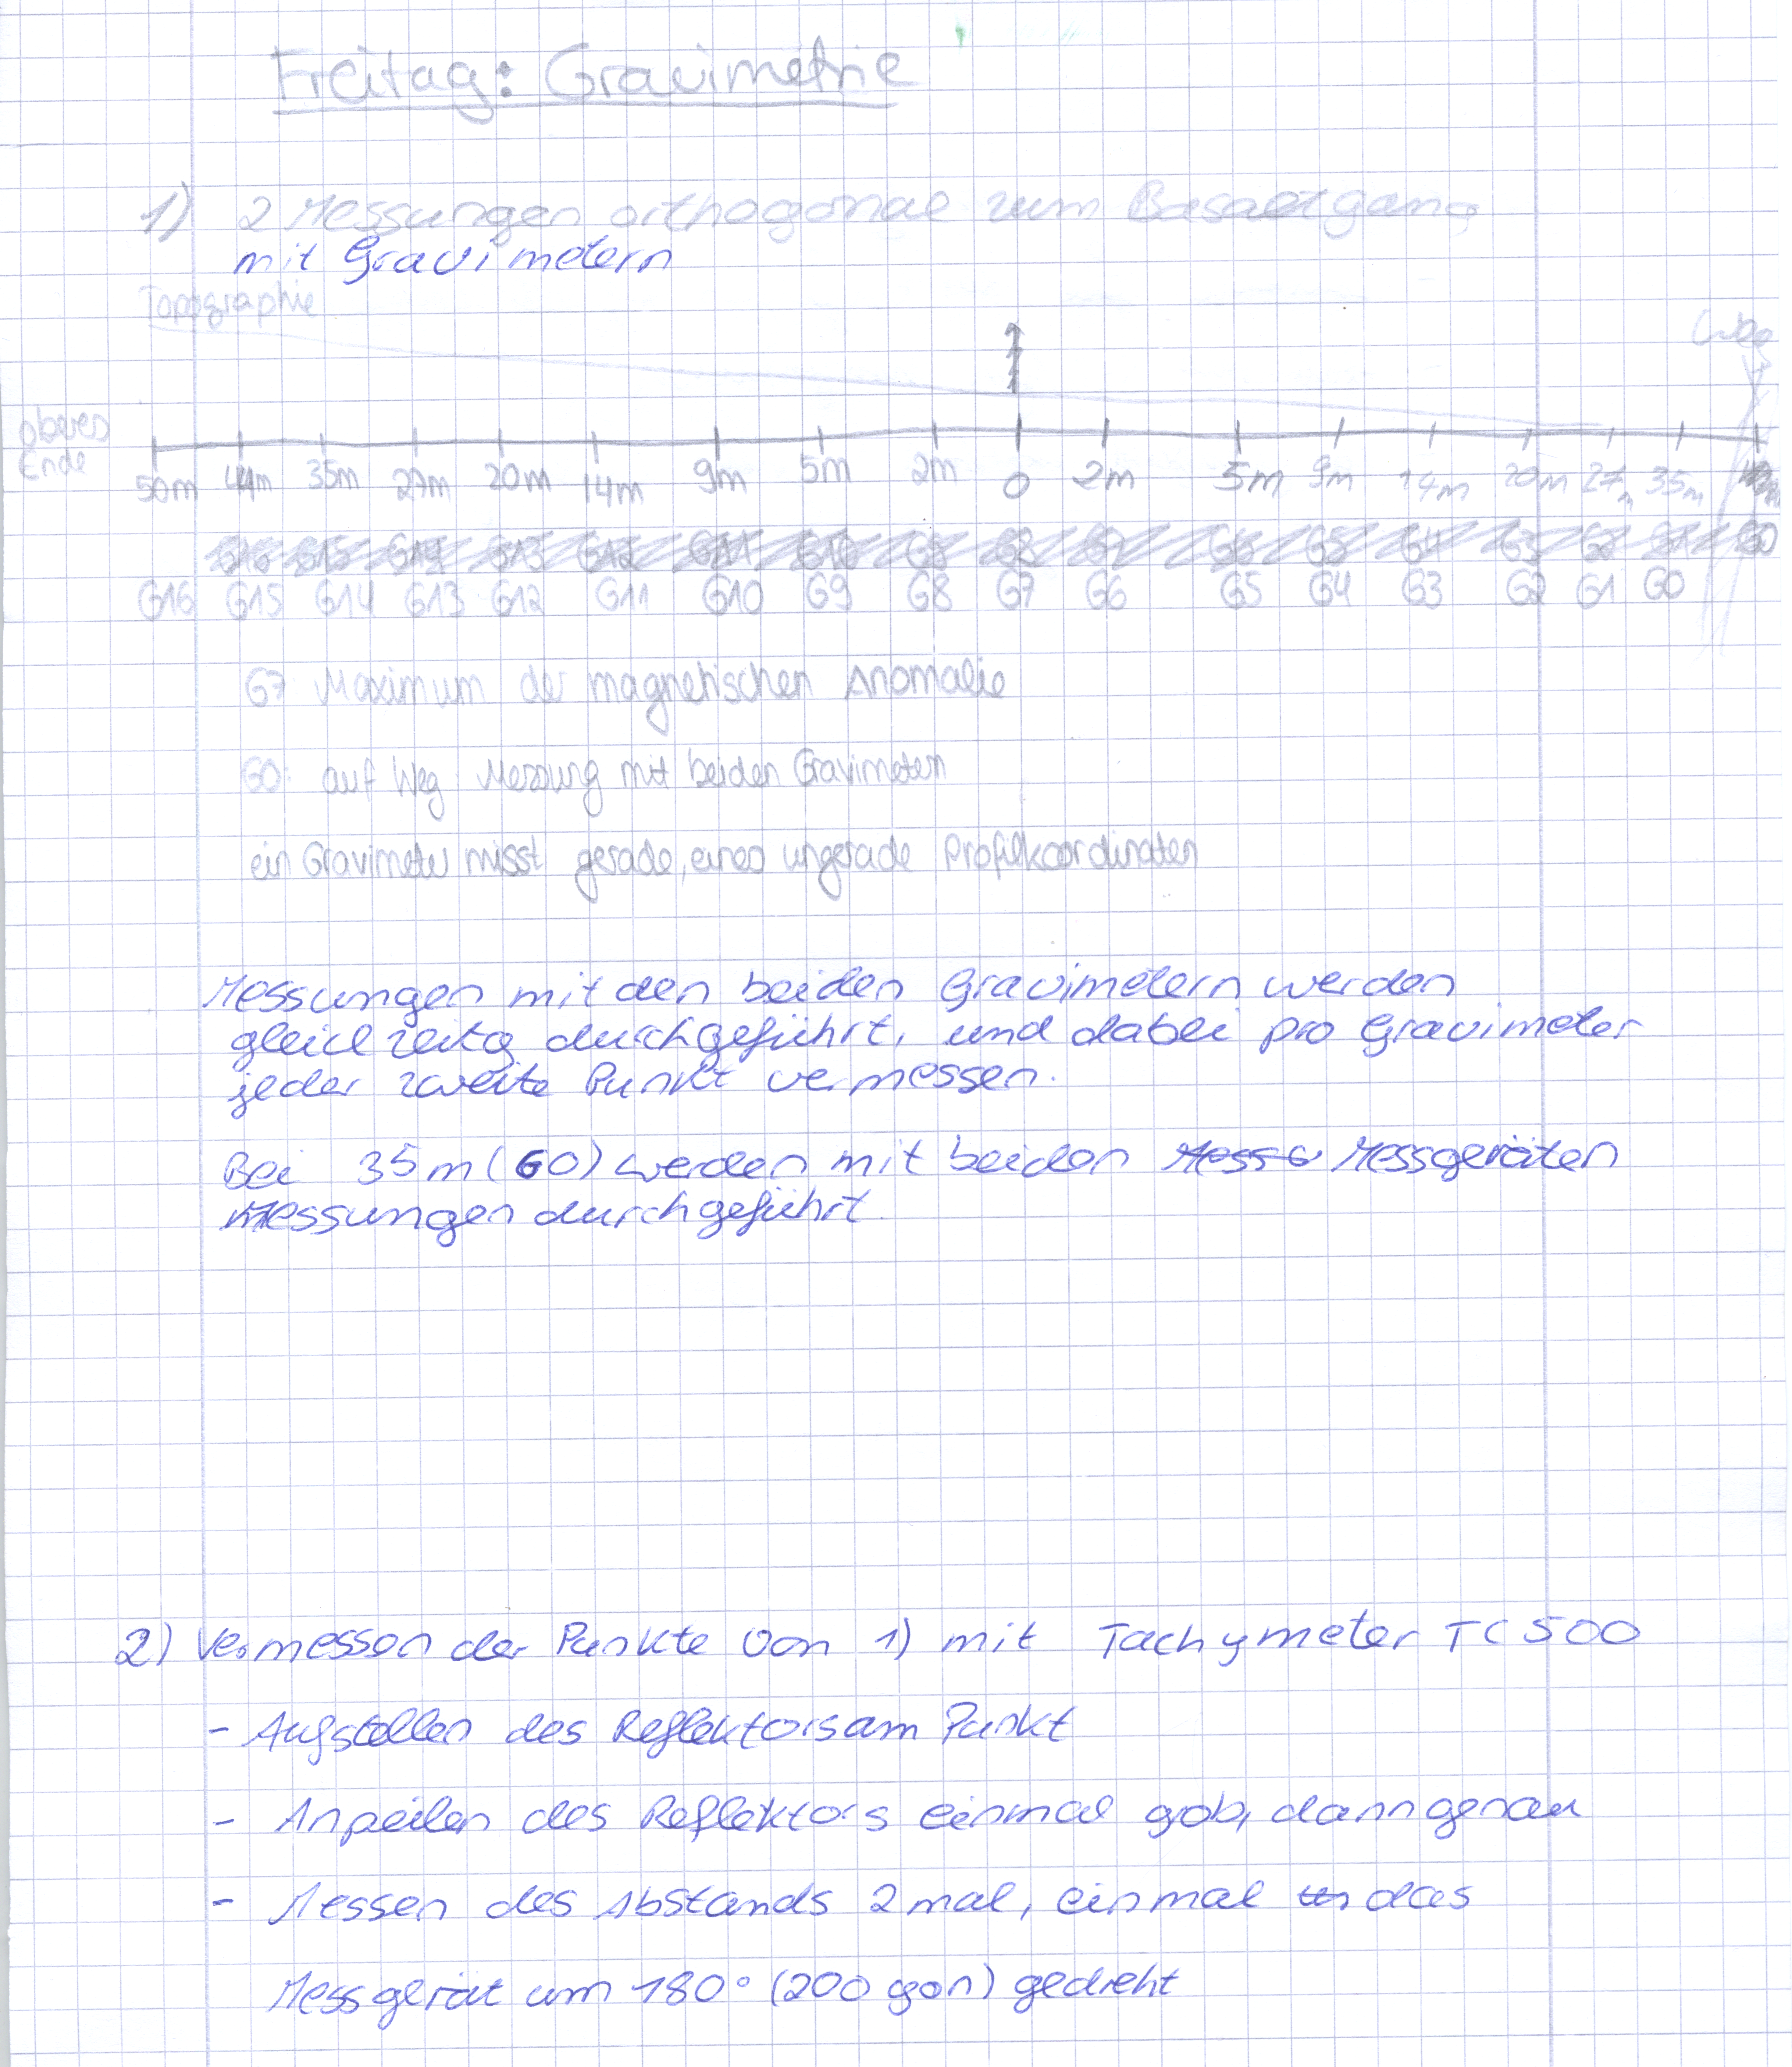
\includegraphics[width=0.9\textwidth]{fig/Messprotokolle/Versuchsbeschreibung1}
 \caption{Versuchsmitschrieb 1}
 \label{fig:mitschrieb1}
\end{figure}

\begin{figure}[!ht]
 \centering
 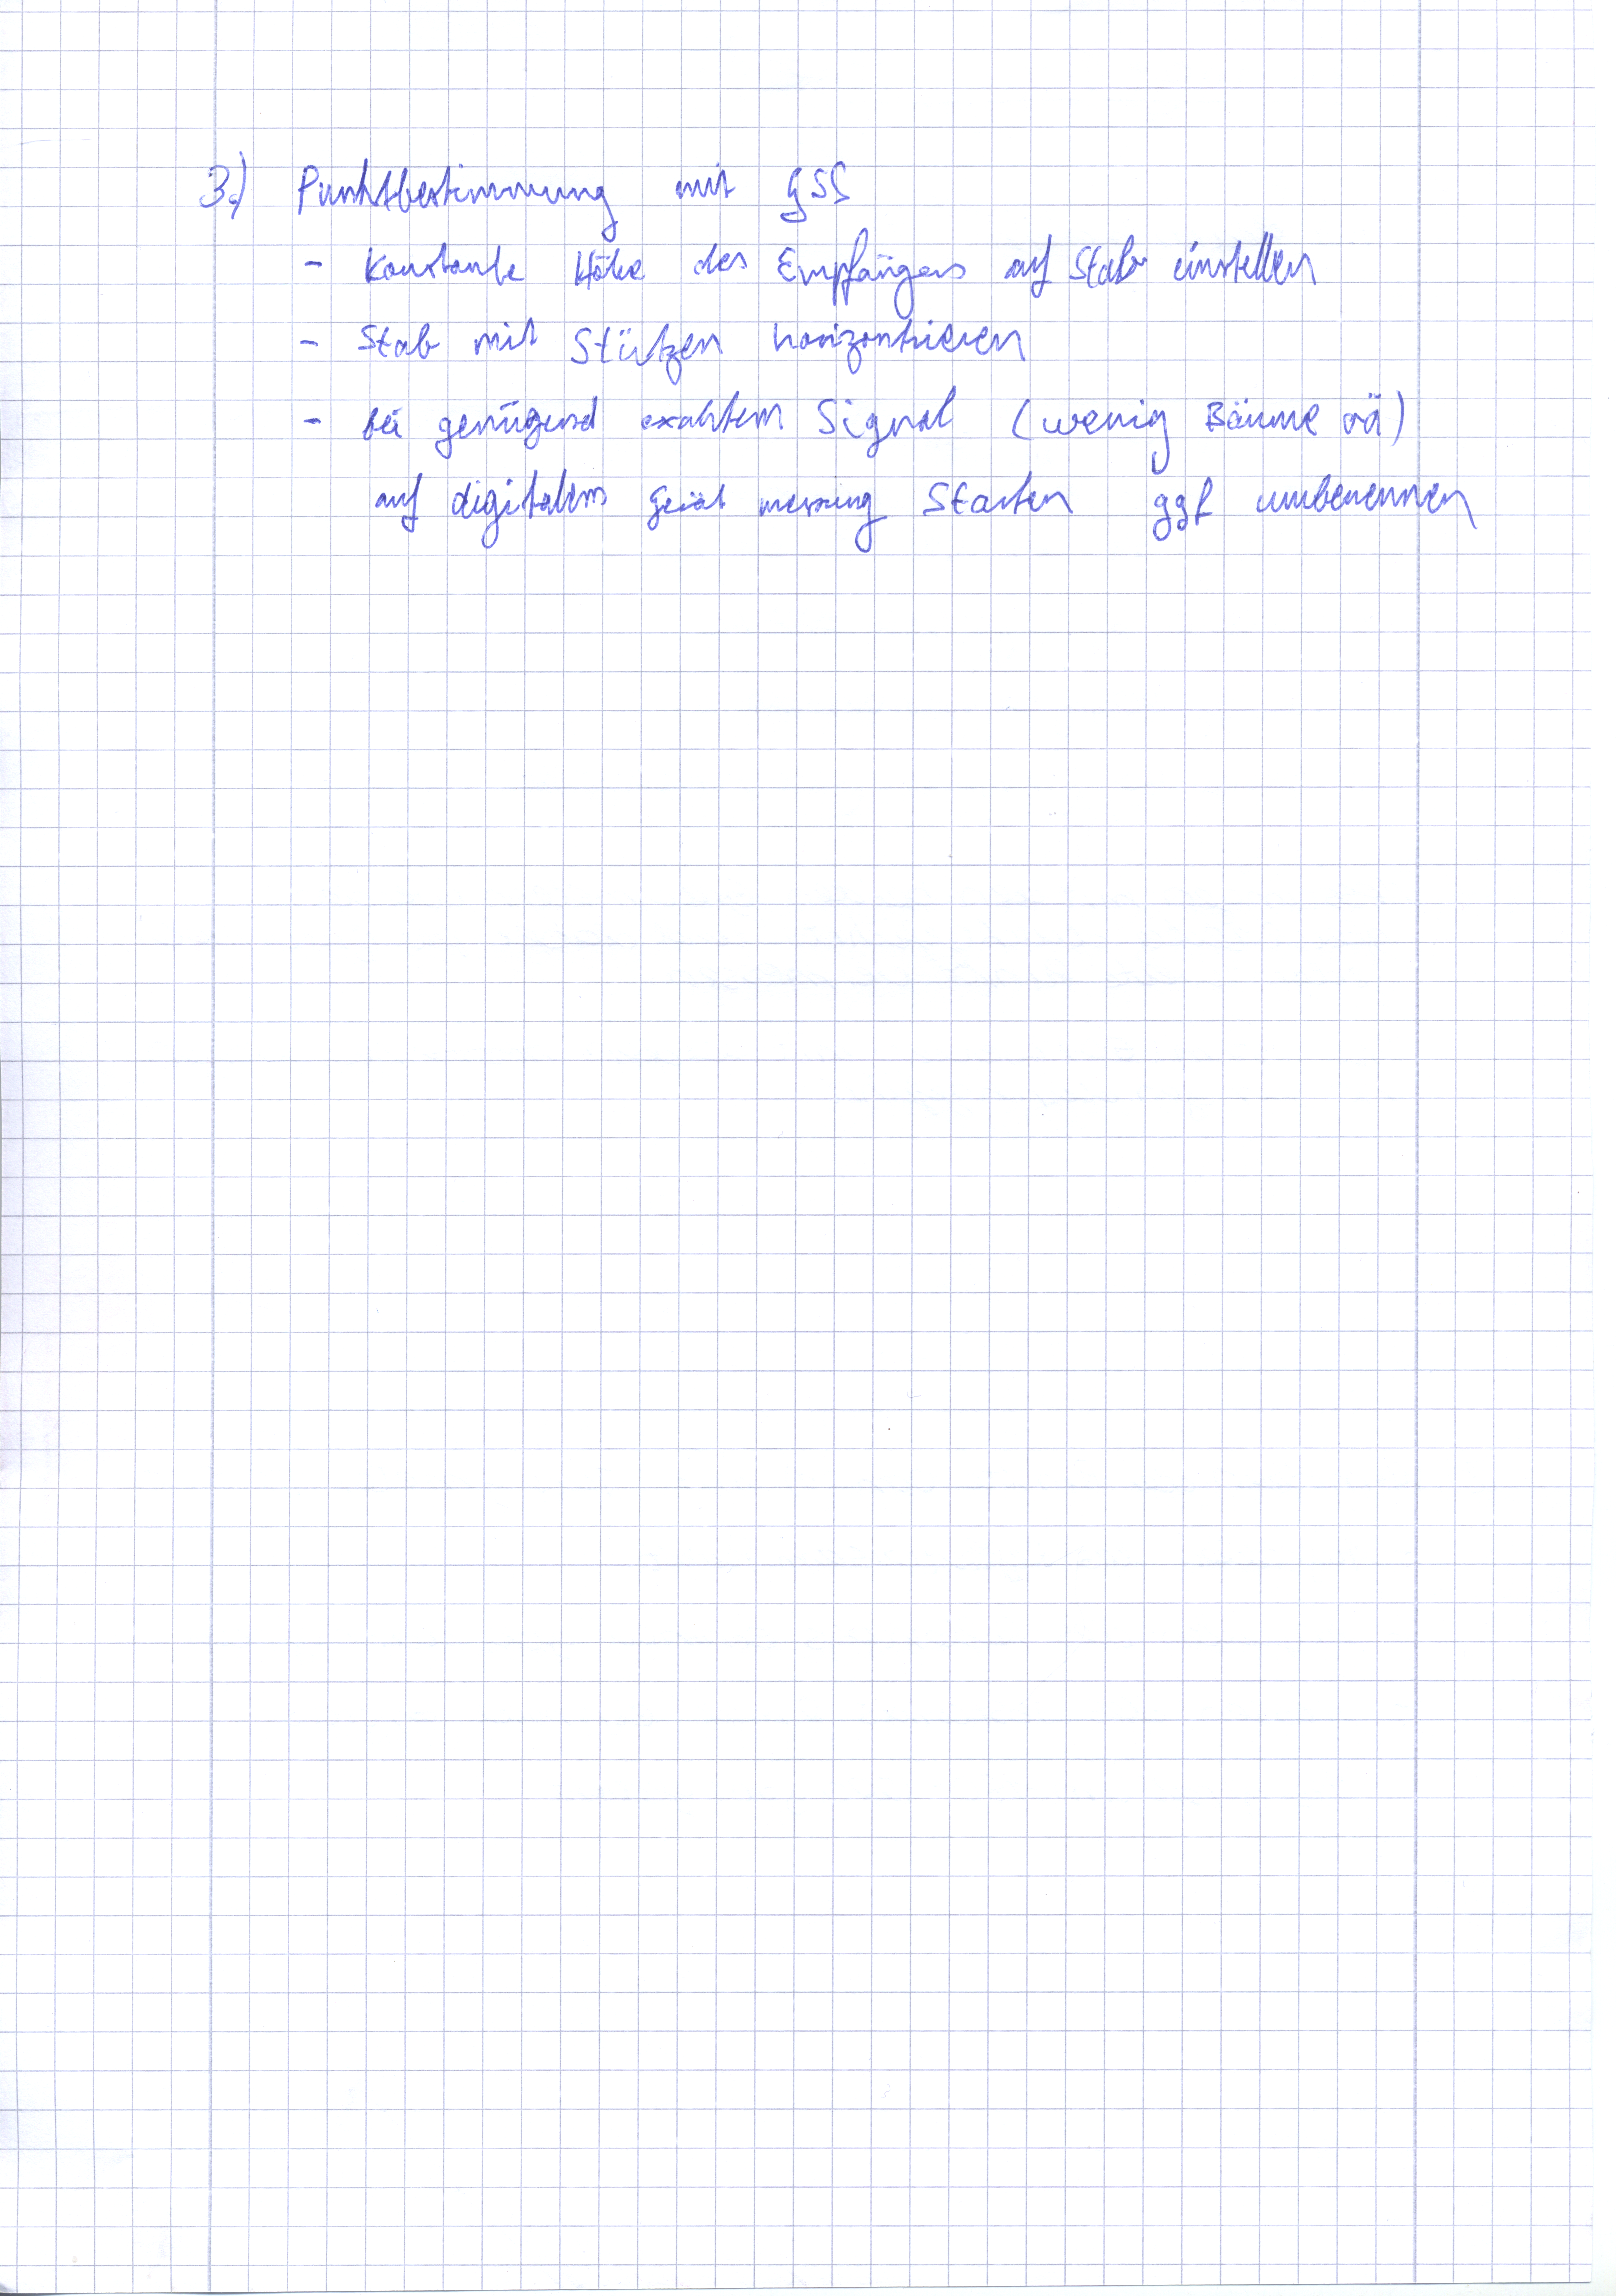
\includegraphics[width=\textwidth]{fig/Messprotokolle/Versuchsbeschreibung2}
 \caption{Versuchsmitschrieb 2}
 \label{fig:mitschrieb2}
\end{figure}

\begin{figure}[!ht]
 \centering
 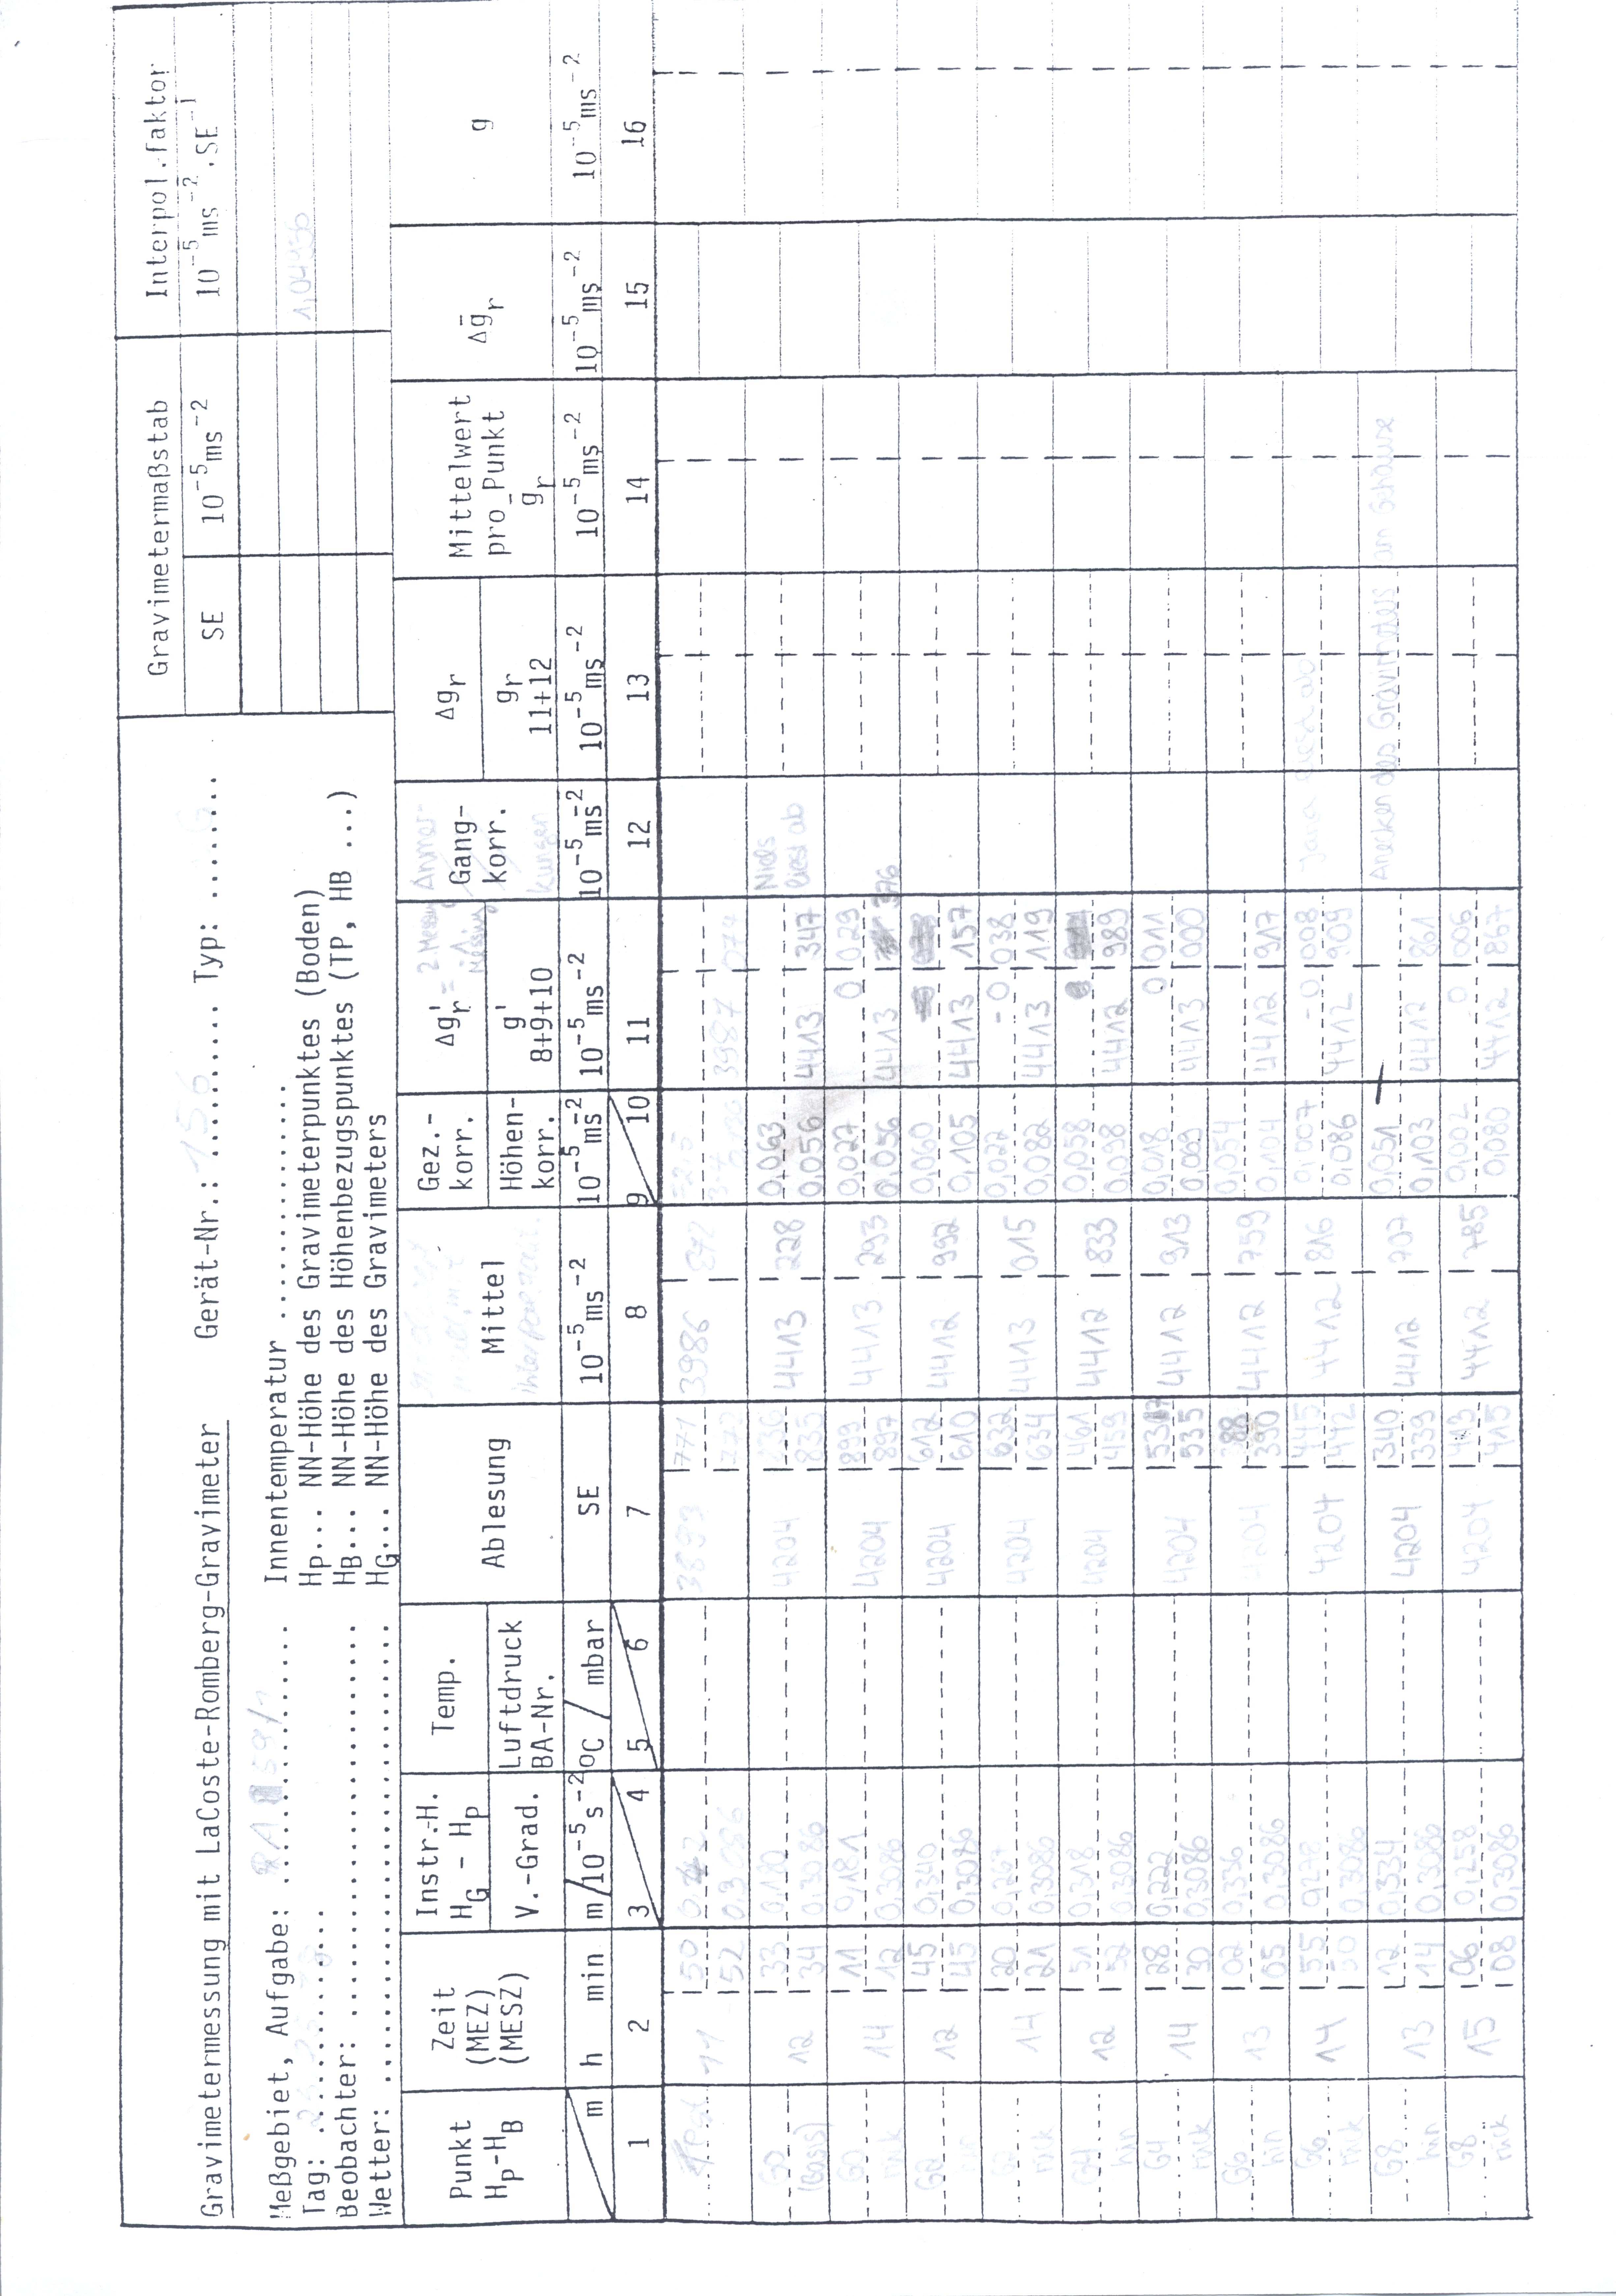
\includegraphics[width=\textwidth]{fig/Messprotokolle/Messprotokoll1-156g}
 \caption{1. Messprotokoll der Messungen mit Gerät Nr. 156 Typ G}
 \label{fig:MP1_156}
\end{figure}

\begin{figure}[!ht]
 \centering
 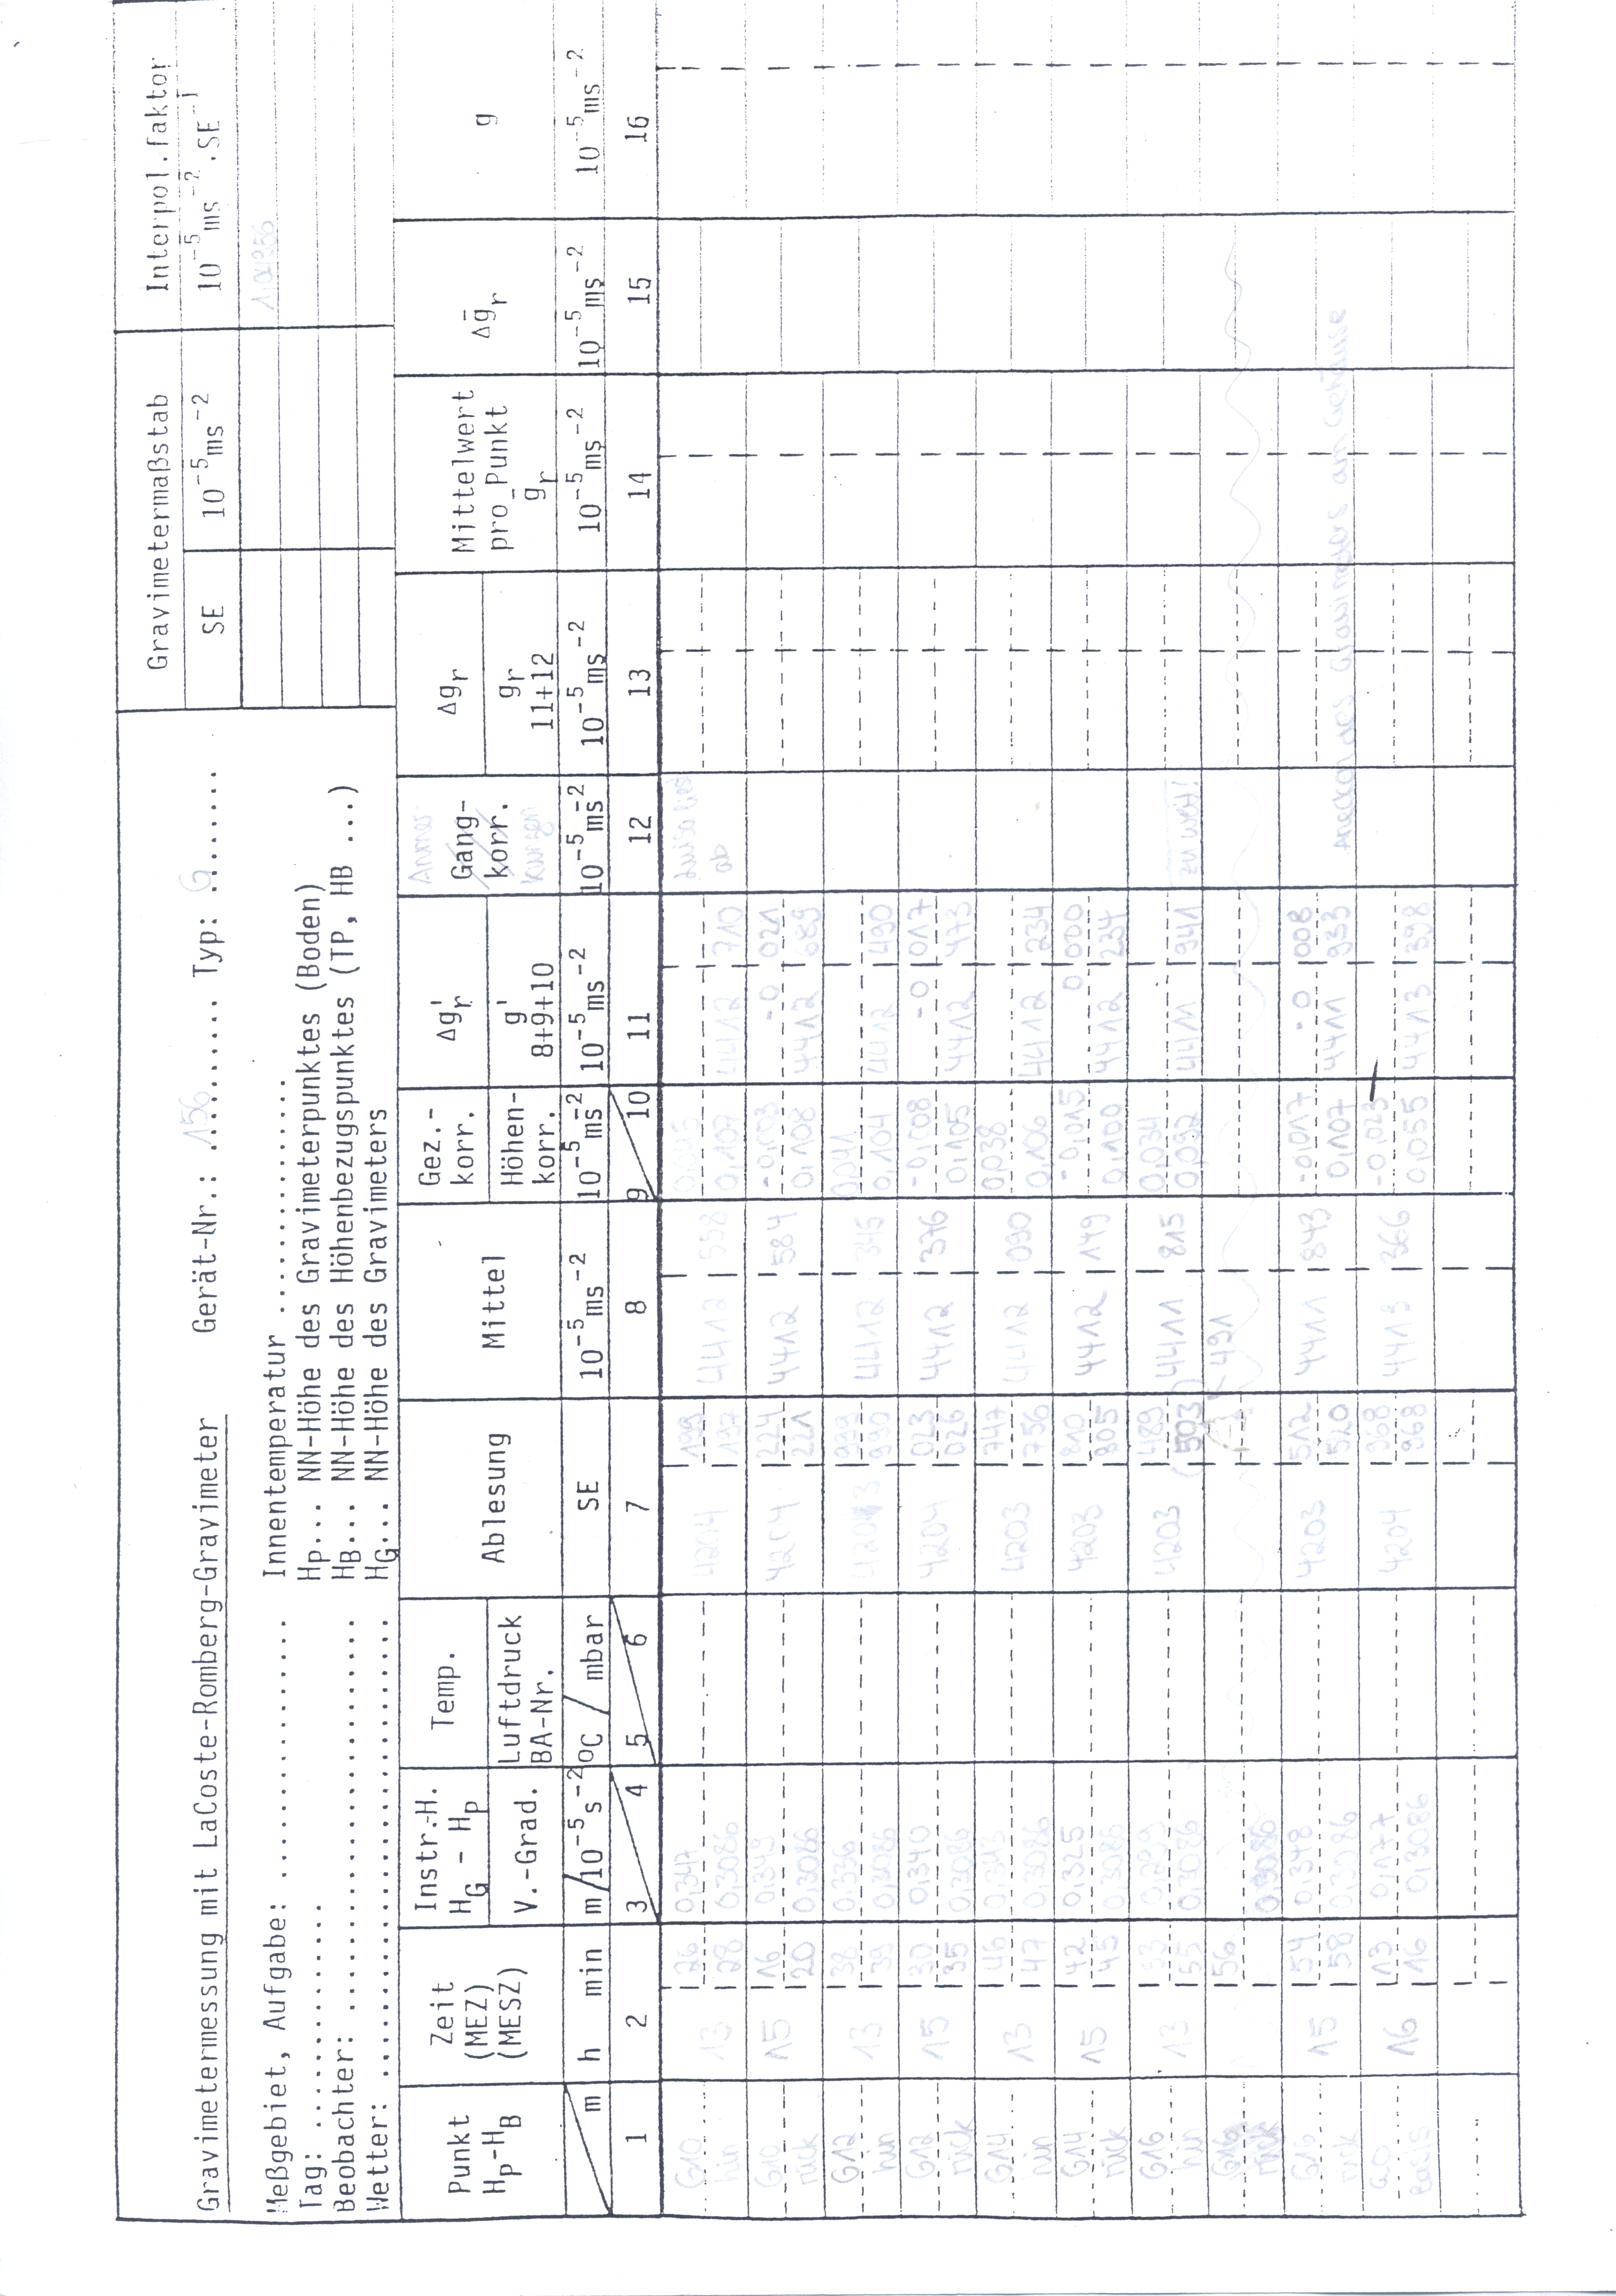
\includegraphics[width=\textwidth]{fig/Messprotokolle/Messprotokoll2-156g}
 \caption{2. Messprotokoll der Messungen mit Gerät Nr. 156 Typ G}
 \label{fig:MP2_156}
\end{figure}

\begin{figure}[!ht]
 \centering
 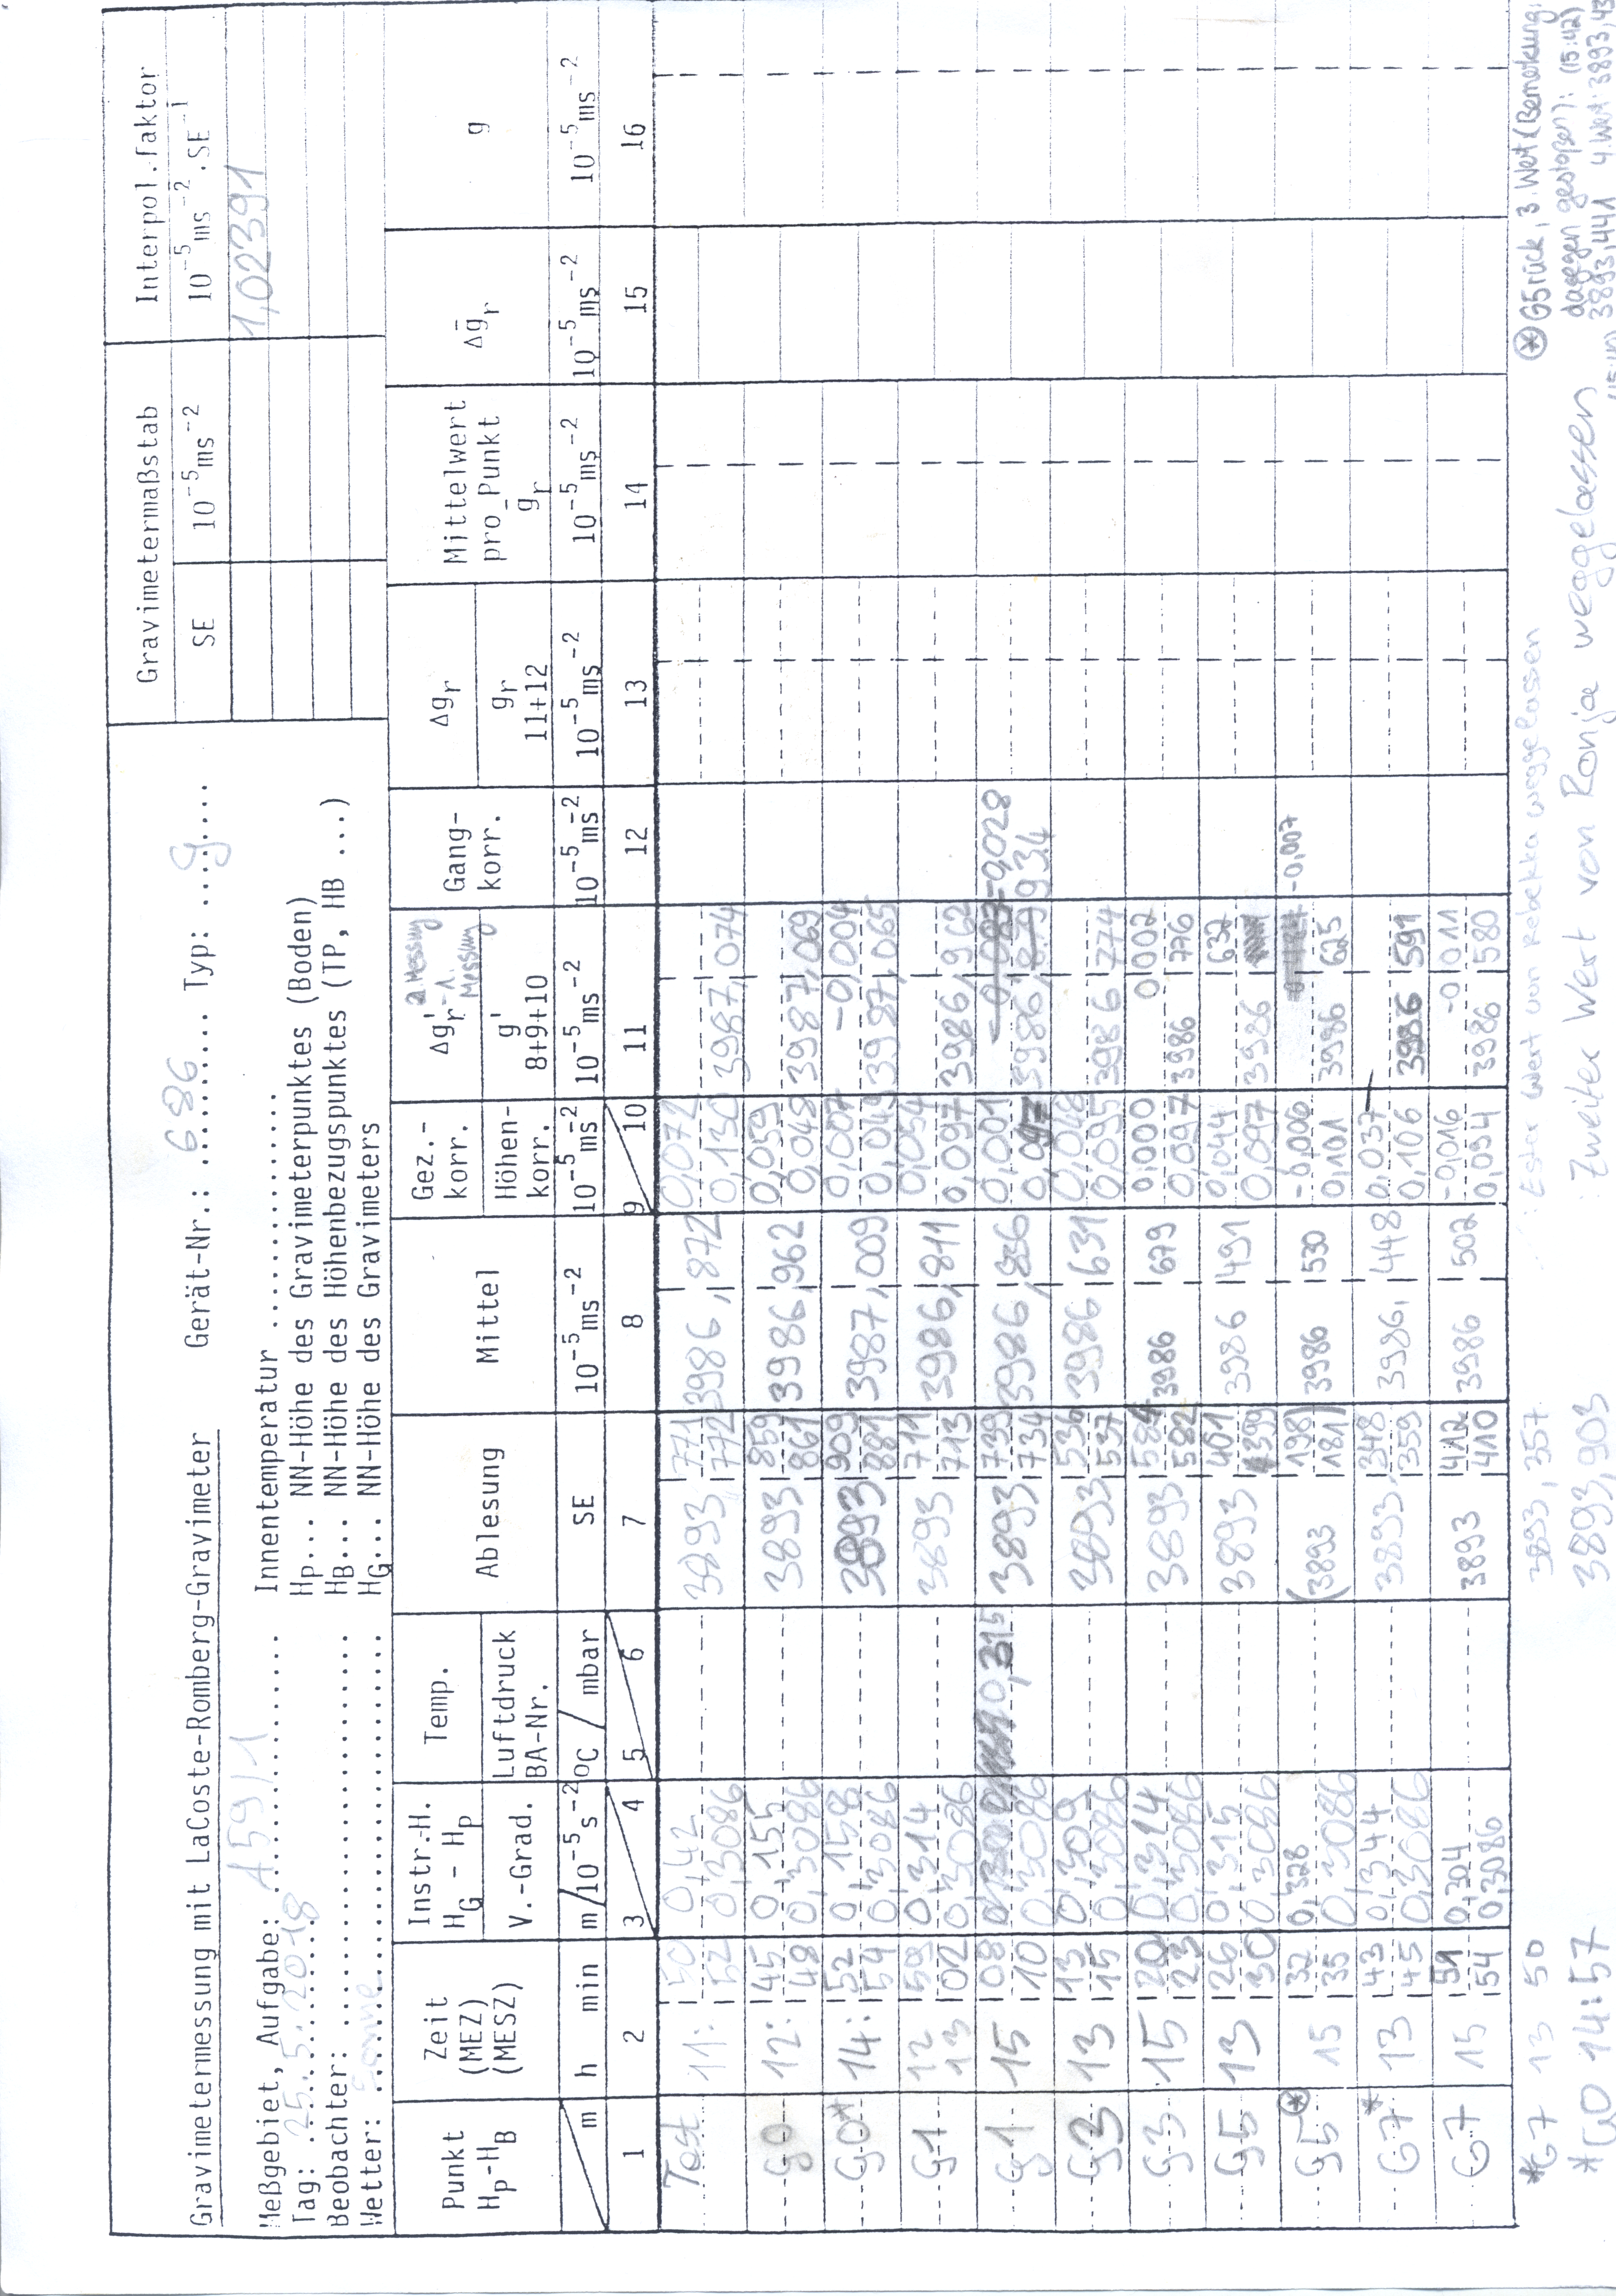
\includegraphics[width=\textwidth]{fig/Messprotokolle/Messprotokoll1-686g}
 \caption{1. Messprotokoll der Messungen mit Gerät Nr. 686 Typ G}
 \label{fig:MP1_686}
\end{figure}

\begin{figure}[!ht]
 \centering
 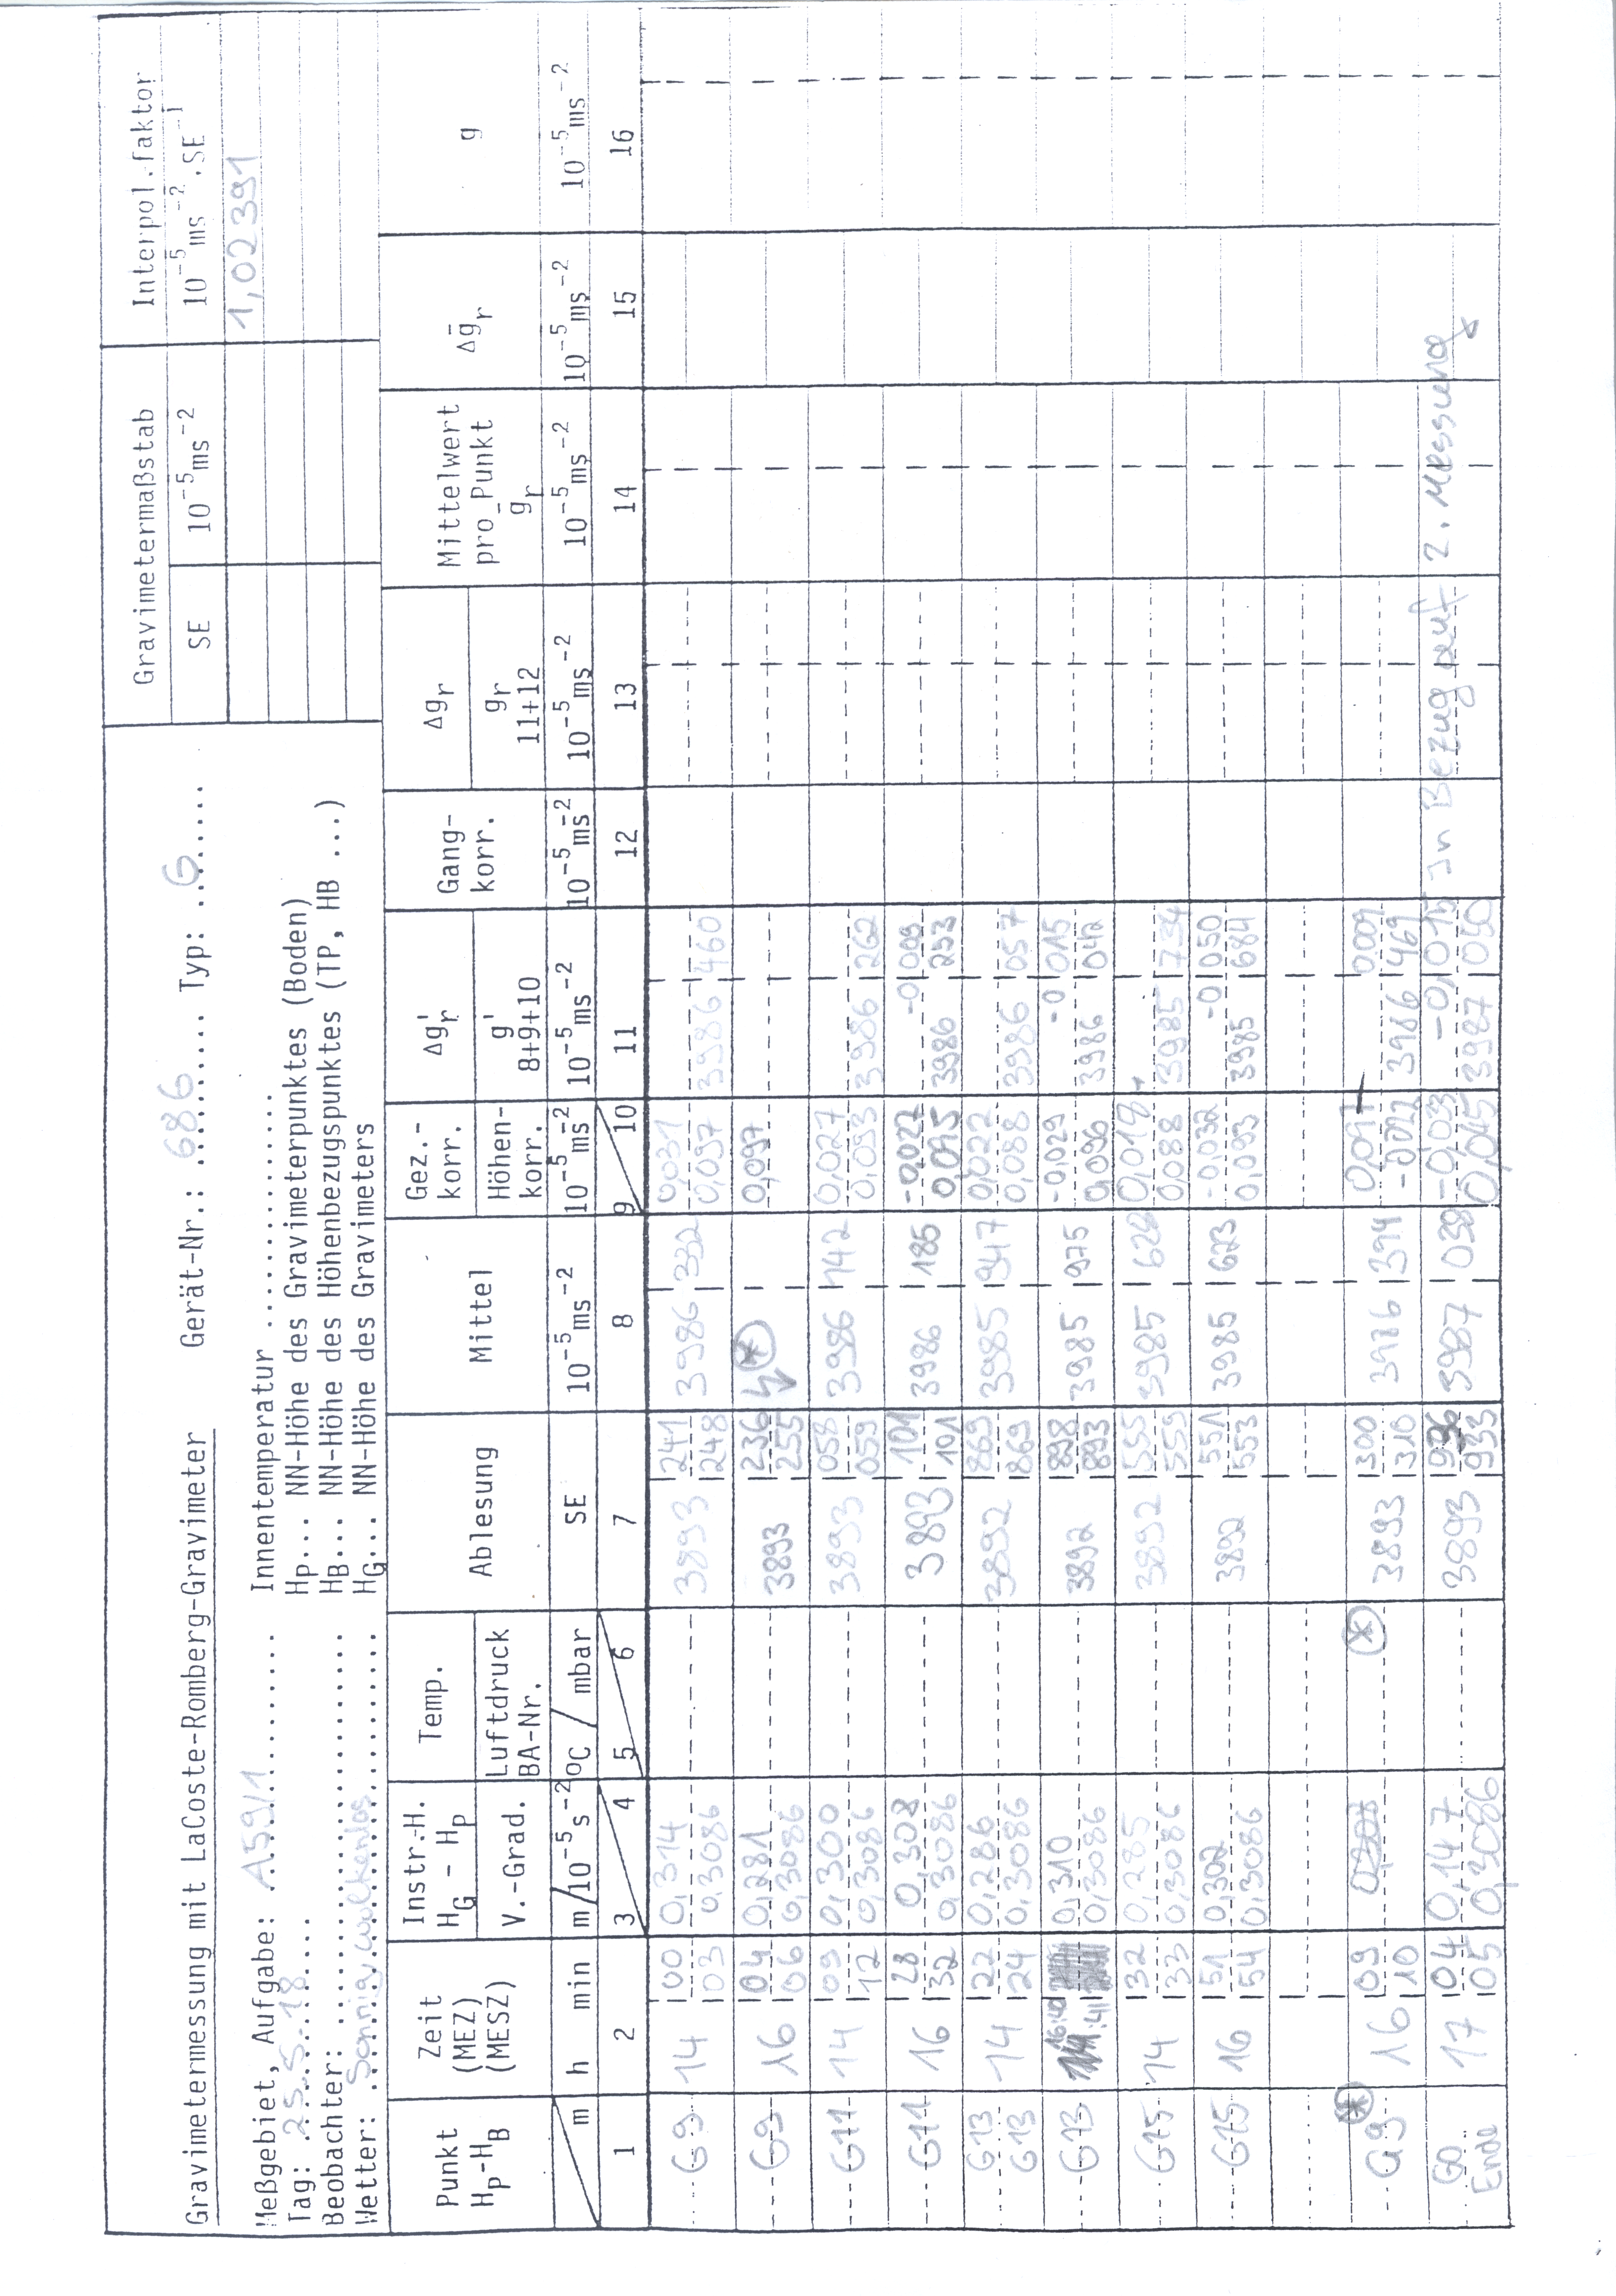
\includegraphics[width=\textwidth]{fig/Messprotokolle/Messprotokoll2-686g}
 \caption{2. Messprotokoll der Messungen mit Gerät Nr. 686 Typ G}
 \label{fig:MP2_686}
\end{figure}

\begin{figure}[!ht]
 \centering
 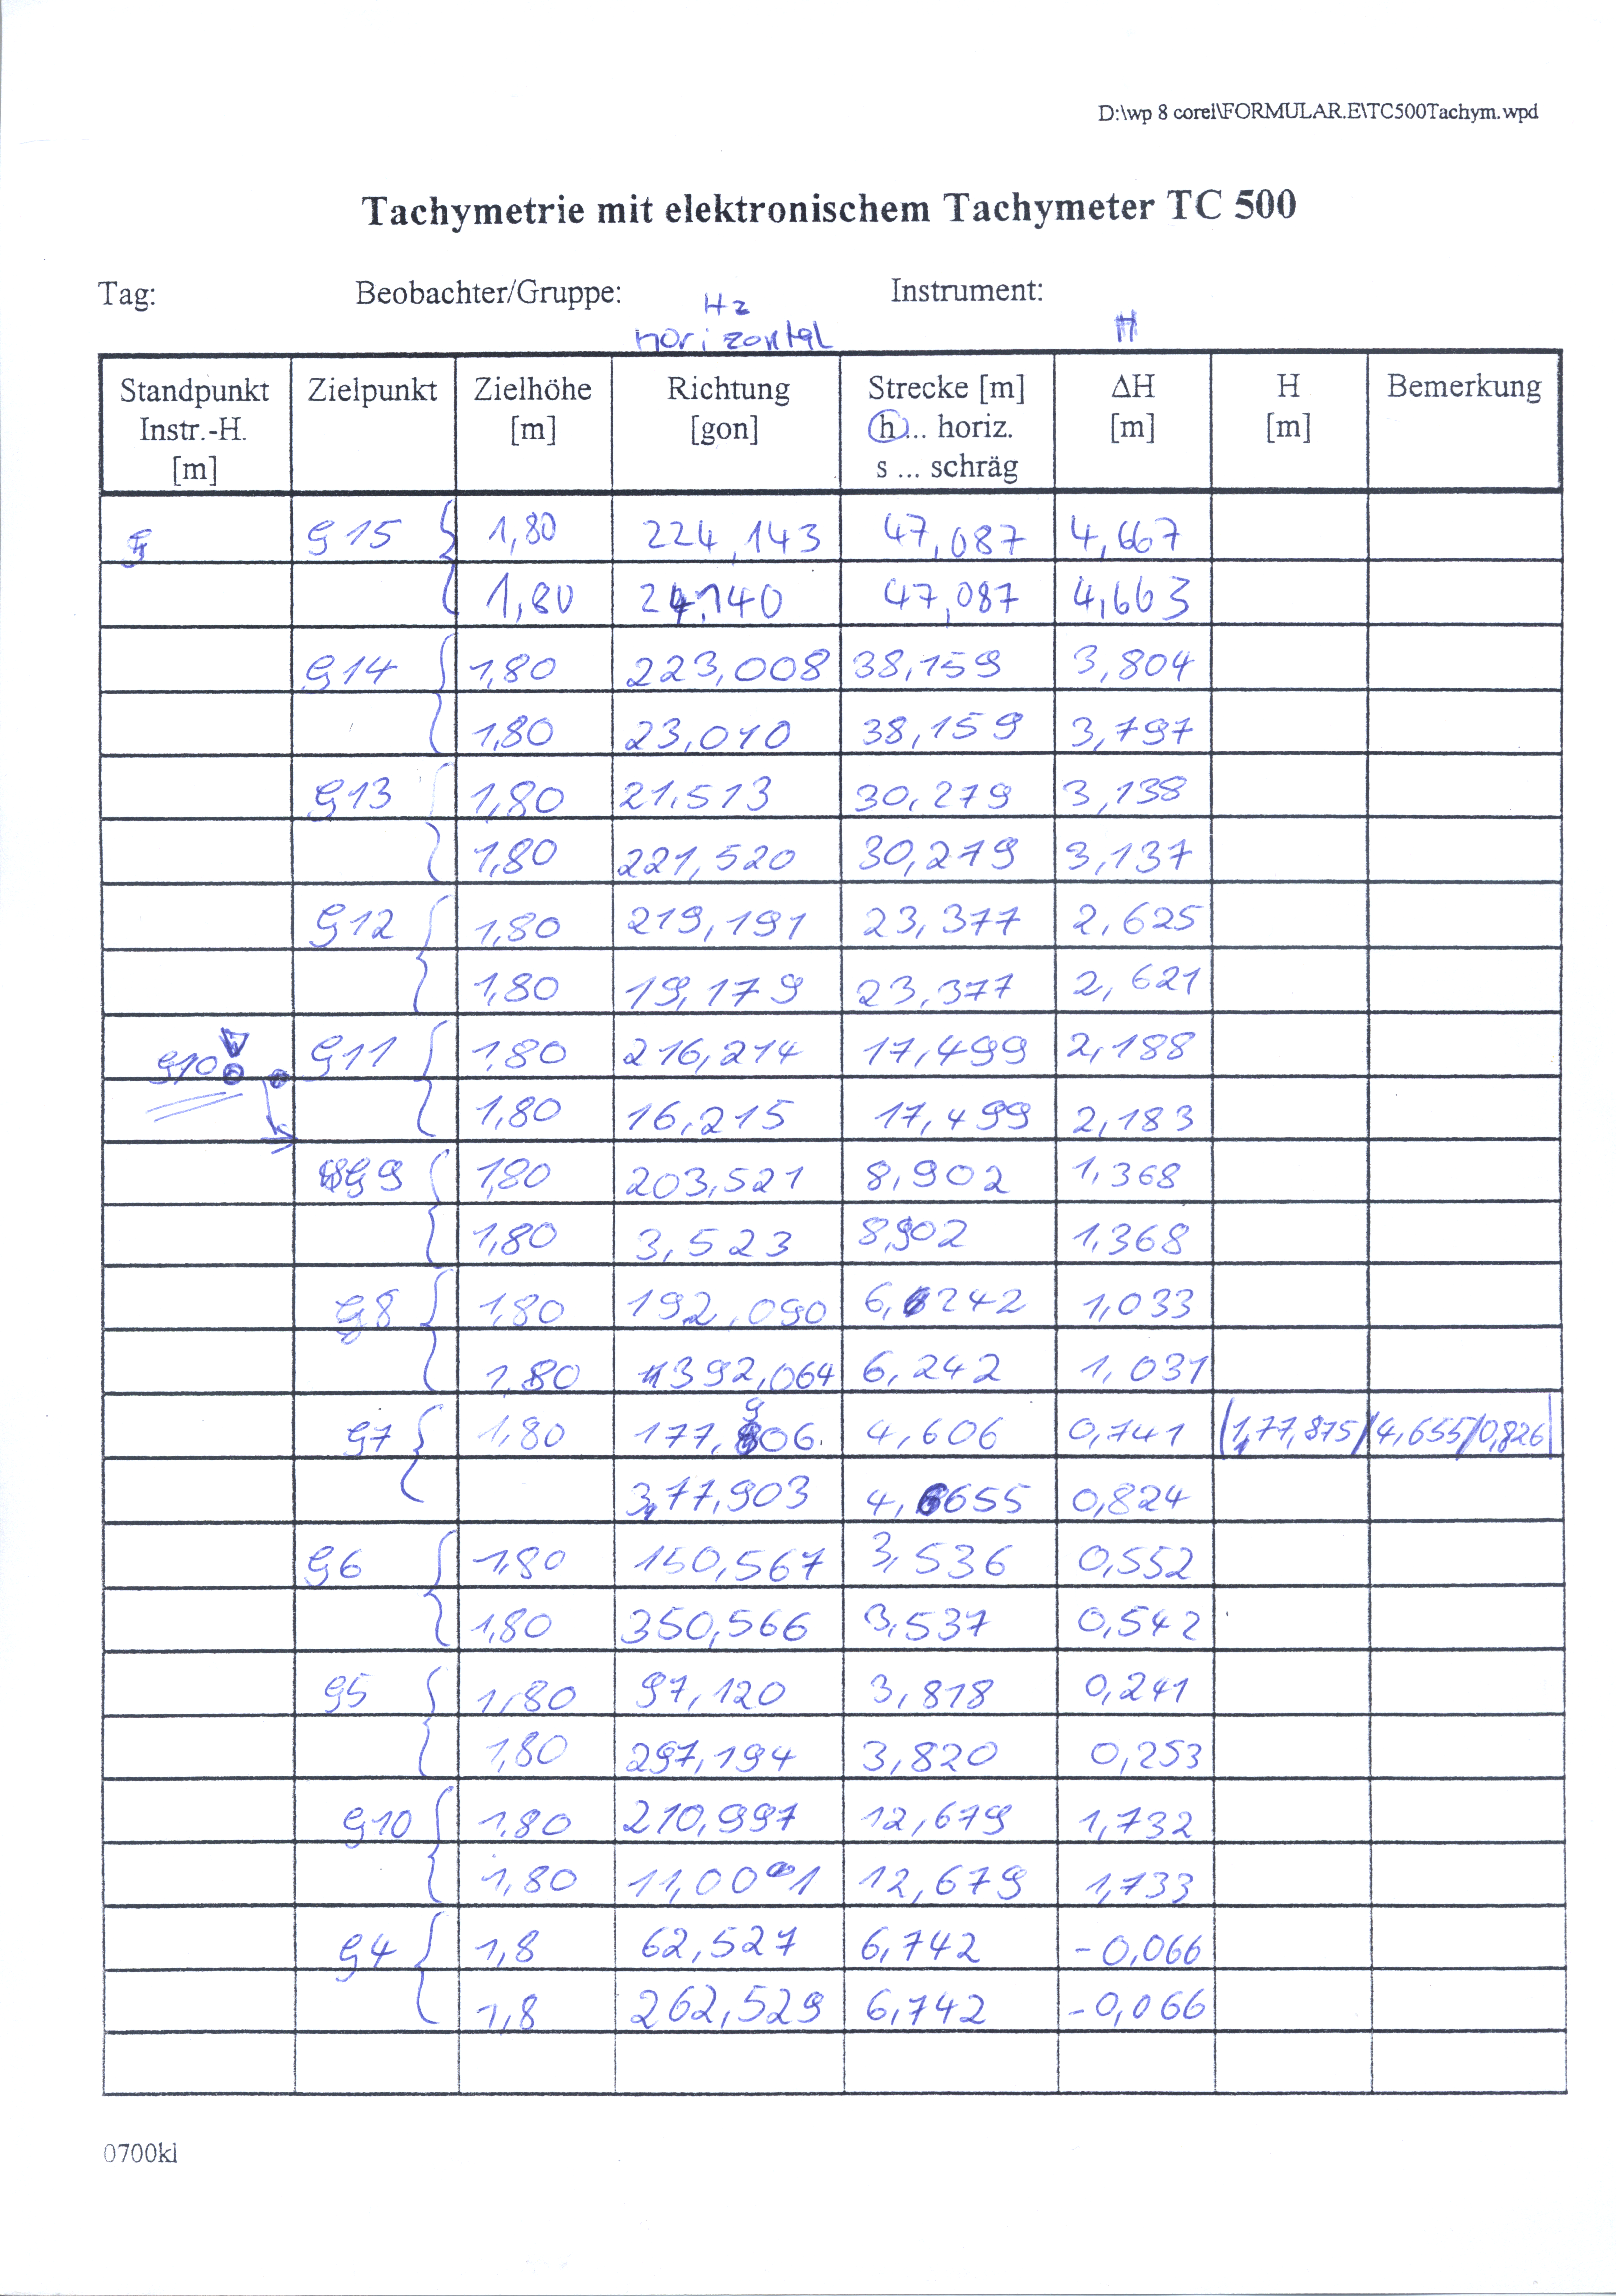
\includegraphics[width=\textwidth]{fig/Messprotokolle/Tachymetrie1}
 \caption{1. Messprotokoll zur Tachymetrie}
 \label{fig:MPTachymetrie1}
\end{figure}

\begin{figure}[!ht]
 \centering
 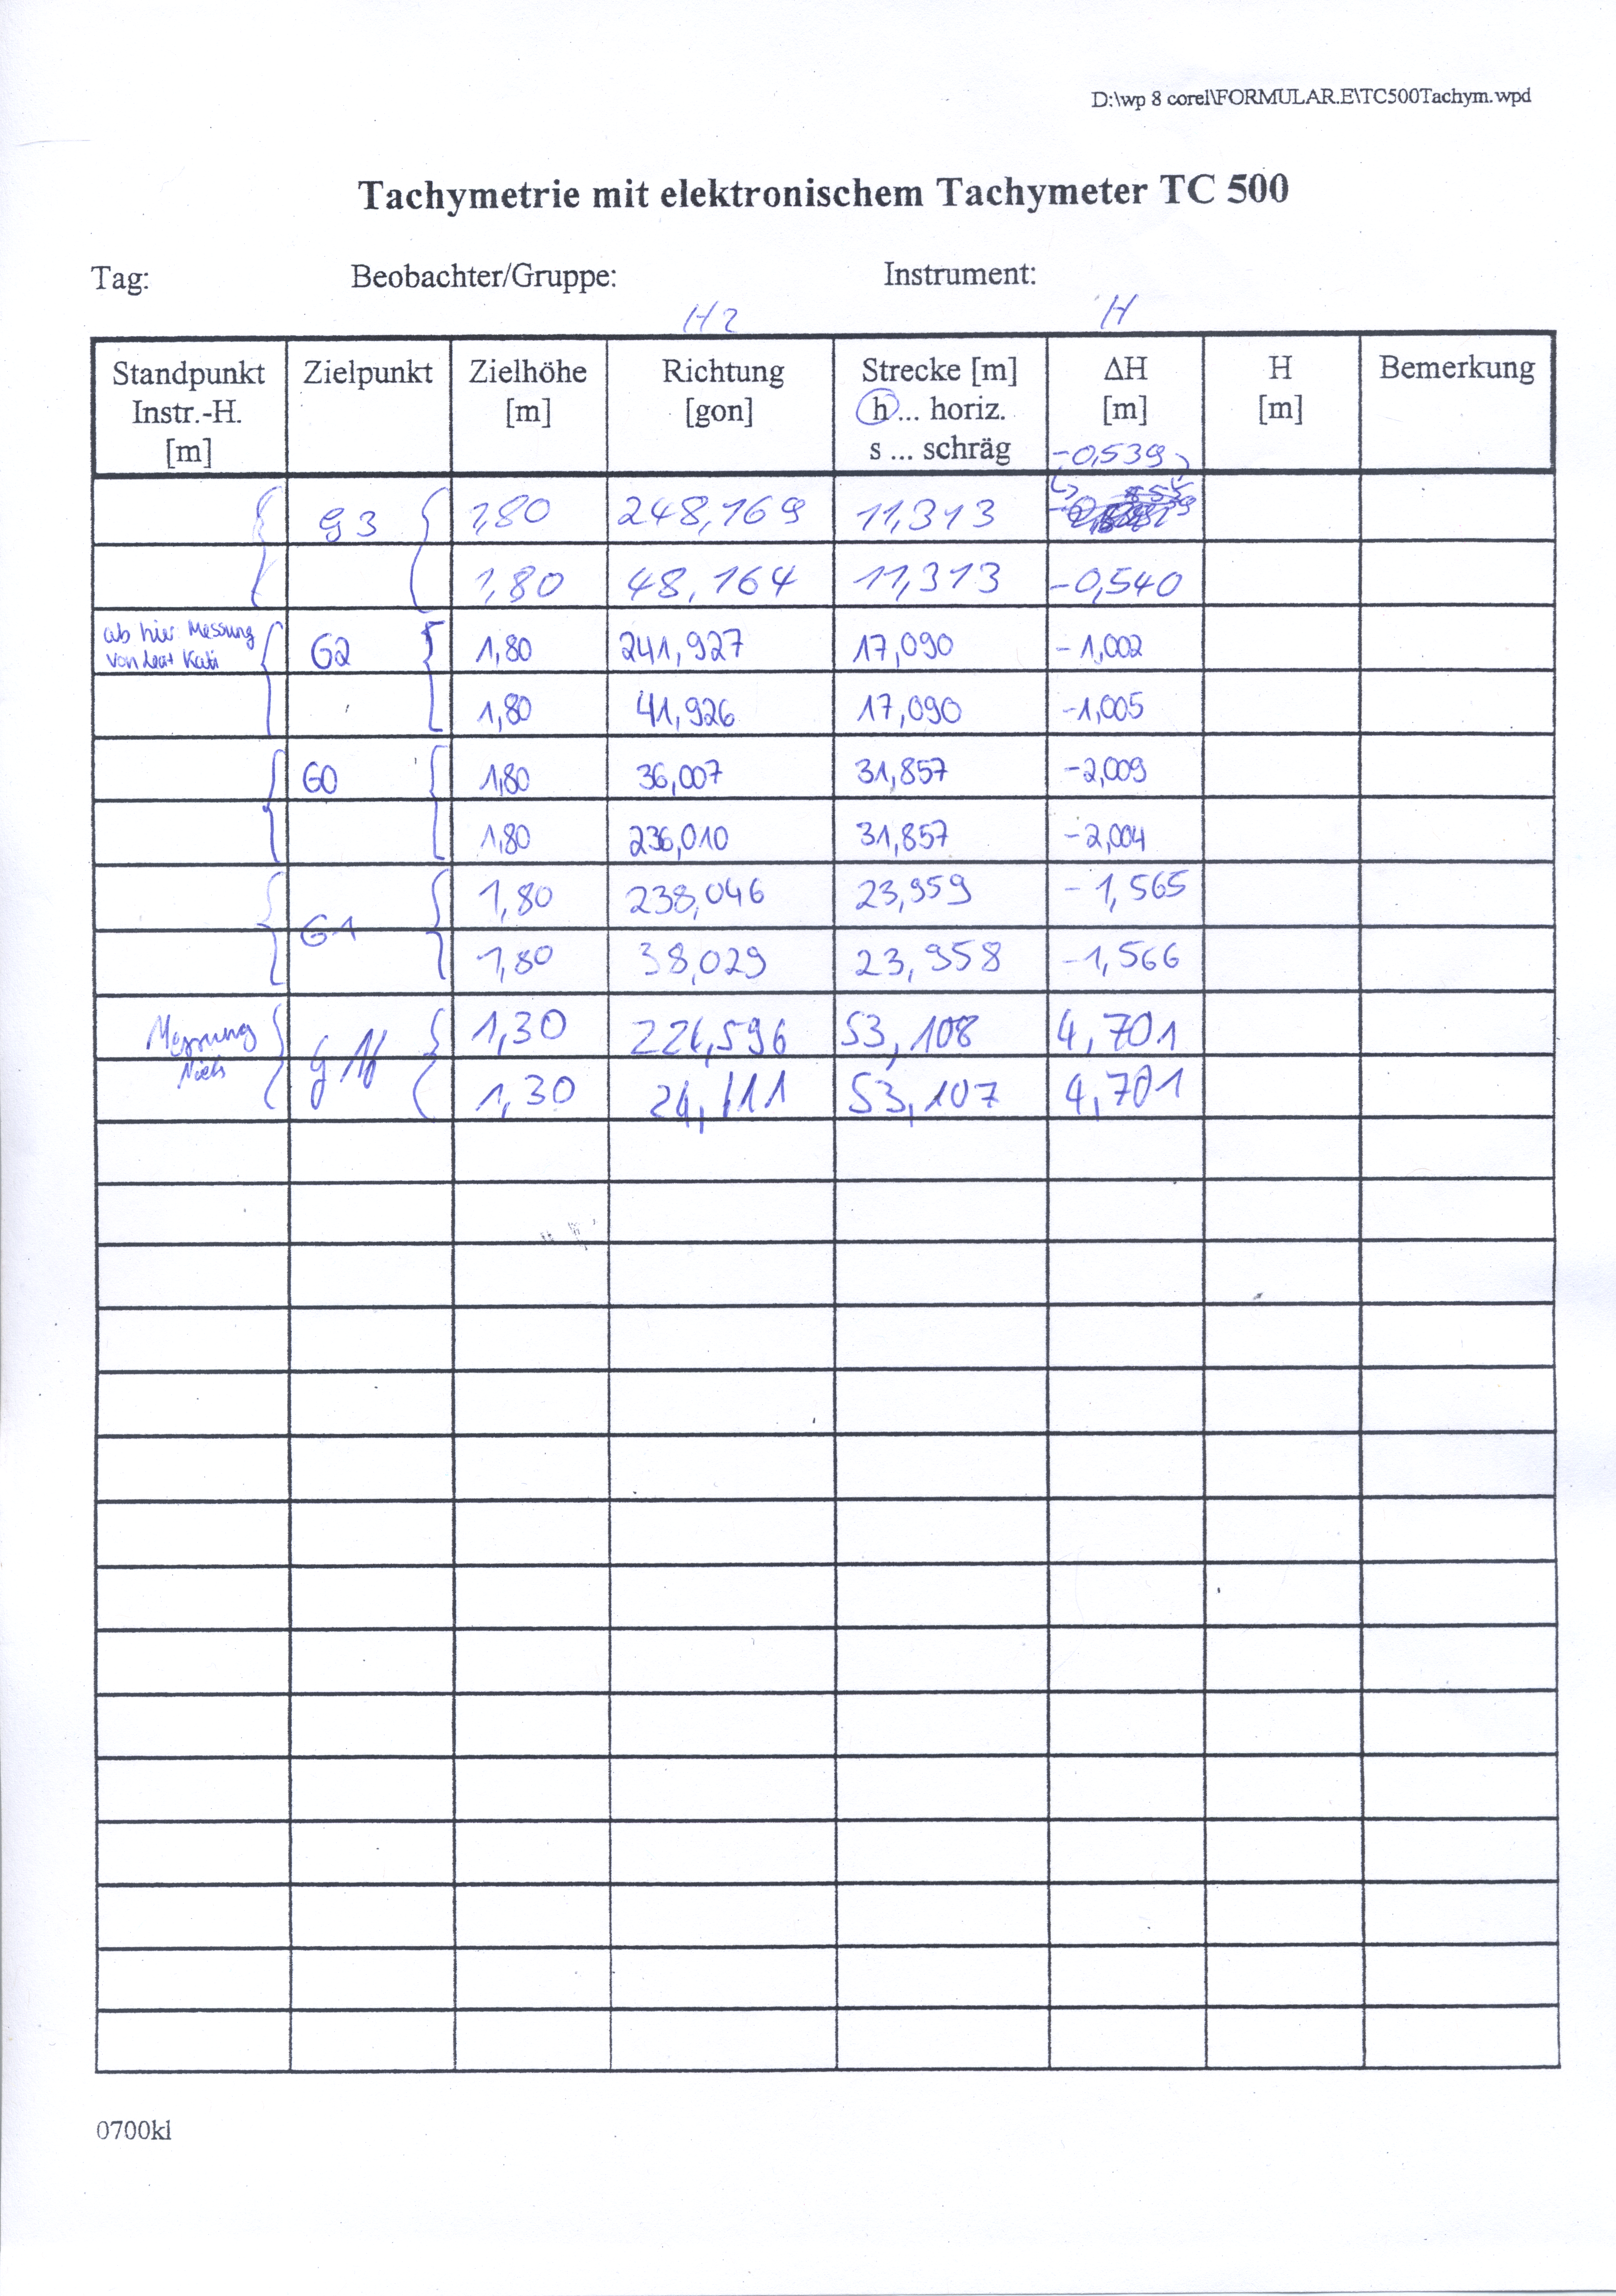
\includegraphics[width=\textwidth]{fig/Messprotokolle/Tachymetrie2}
 \caption{1. Messprotokoll zur Tachymetrie}
 \label{fig:MPTachymetrie2}
\end{figure}

\FloatBarrier
\section{Messergebnisse}

\begin{table}[!ht]
\centering
\caption{Teil 1 der Ergebnisse der GPS-Vermessung}
\label{tab:gps1}
\begin{tabular}{lllllll}
\toprule
Name    & Lon(East)   & Lat(North)   & Ht       & Ht(G)    & Date       & Time     \\
\midrule
S11     & 8.757259947 & 47.768672362 & 590.6016 & 590.6016 & 2018-05-25 & 13:06:15 \\
S13     & 8.757859174 & 47.768857824 & 590.4168 & 590.4168 & 2018-05-25 & 13:10:05 \\
S14     & 8.758436670 & 47.769032070 & 593.2414 & 593.2414 & 2018-05-25 & 13:12:26 \\
S12     & 8.758938739 & 47.769196631 & 592.2514 & 592.2514 & 2018-05-25 & 13:14:16 \\
E21     & 8.756625846 & 47.768510899 & 589.4322 & 589.4322 & 2018-05-25 & 13:18:53 \\
E22     & 8.759064096 & 47.769235580 & 591.6336 & 591.6336 & 2018-05-25 & 13:38:14 \\
G0      & 8.753717653 & 47.766529817 & 562.3773 & 562.3773 & 2018-05-25 & 14:00:40 \\
G1      & 8.753810544 & 47.766564339 & 562.8301 & 562.8301 & 2018-05-25 & 14:05:10 \\
G2      & 8.753891246 & 47.766595629 & 563.4272 & 563.4272 & 2018-05-25 & 14:07:08 \\
G3      & 8.753963012 & 47.766618050 & 563.7453 & 563.7453 & 2018-05-25 & 14:11:09 \\
G4      & 8.754018082 & 47.766644131 & 564.3878 & 564.3878 & 2018-05-25 & 14:17:03 \\
G5      & 8.754063775 & 47.766661286 & 564.7339 & 564.7339 & 2018-05-25 & 14:19:38 \\
G6      & 8.754099169 & 47.766674250 & 565.0490 & 565.0490 & 2018-05-25 & 14:22:27 \\
G7      & 8.754122690 & 47.766683198 & 565.2543 & 565.2543 & 2018-05-25 & 14:25:25 \\
G8      & 8.754145448 & 47.766692940 & 565.4319 & 565.4319 & 2018-05-25 & 14:27:49 \\
G9      & 8.754179516 & 47.766706224 & 565.7621 & 565.7621 & 2018-05-25 & 14:30:52 \\
G10     & 8.754225023 & 47.766724489 & 566.1333 & 566.1333 & 2018-05-25 & 14:34:27 \\
G11     & 8.754282894 & 47.766746486 & 566.5949 & 566.5949 & 2018-05-25 & 14:36:44 \\
G12     & 8.754351400 & 47.766773616 & 567.0370 & 567.0370 & 2018-05-25 & 14:38:37 \\
G13     & 8.754432441 & 47.766804206 & 567.5562 & 567.5562 & 2018-05-25 & 14:40:08 \\
G14     & 8.754524035 & 47.766839825 & 568.2036 & 568.2036 & 2018-05-25 & 14:42:26 \\
G15     & 8.754627906 & 47.766879777 & 569.1020 & 569.1020 & 2018-05-25 & 14:44:56 \\
G16     & 8.754697912 & 47.766906922 & 569.6233 & 569.6233 & 2018-05-25 & 14:46:44 \\
G4bup   & 8.754018242 & 47.766643862 & 564.3500 & 564.3500 & 2018-05-25 & 14:55:46 \\
G3bup   & 8.753960912 & 47.766621604 & 563.8981 & 563.8981 & 2018-05-25 & 14:56:51 \\
m basis & 8.752734929 & 47.767417892 & 579.3217 & 579.3217 & 2018-05-25 & 15:14:00 \\
S21     & 8.753971287 & 47.766861593 & 567.1719 & 567.1719 & 2018-05-25 & 15:50:06 \\
M1      & 8.753887975 & 47.766798997 & 566.1727 & 566.1727 & 2018-05-25 & 15:54:11 \\
M4      & 8.753755419 & 47.766546207 & 562.6191 & 562.6191 & 2018-05-25 & 15:59:29 \\
E11     & 8.753758139 & 47.766544486 & 562.6028 & 562.6028 & 2018-05-25 & 16:04:35 \\
M24     & 8.753938600 & 47.766595287 & 563.3535 & 563.3535 & 2018-05-25 & 16:07:16 \\
M21     & 8.753922700 & 47.766608115 & 563.5182 & 563.5182 & 2018-05-25 & 16:08:23 \\
M22     & 8.753908722 & 47.766624980 & 563.6719 & 563.6719 & 2018-05-25 & 16:09:25 \\
M28     & 8.753920701 & 47.766644414 & 563.9703 & 563.9703 & 2018-05-25 & 16:10:49 \\
M29     & 8.754282539 & 47.766682749 & 565.6981 & 565.6981 & 2018-05-25 & 16:12:36 \\
M25     & 8.754291215 & 47.766728209 & 566.2778 & 566.2778 & 2018-05-25 & 16:13:55 \\
M2      & 8.754278175 & 47.766743496 & 566.4378 & 566.4378 & 2018-05-25 & 16:15:45 \\
M23     & 8.754258391 & 47.766758244 & 566.5787 & 566.5787 & 2018-05-25 & 16:16:52 \\
M27     & 8.754428930 & 47.766730977 & 566.5148 & 566.5148 & 2018-05-25 & 16:19:35 \\
M3      & 8.754148748 & 47.766500369 & 562.9455 & 562.9455 & 2018-05-25 & 16:21:31 \\
M26     & 8.754085876 & 47.766598253 & 563.8740 & 563.8740 & 2018-05-25 & 16:23:53 \\
S22     & 8.754241271 & 47.766534642 & 563.7173 & 563.7173 & 2018-05-25 & 16:25:37 \\
S32     & 8.755205319 & 47.766637774 & 565.0036 & 565.0036 & 2018-05-25 & 16:32:15 \\
S31     & 8.754800319 & 47.766890040 & 569.3073 & 569.3073 & 2018-05-25 & 16:36:07 \\
E12     & 8.754461728 & 47.766814484 & 567.6117 & 567.6117 & 2018-05-25 & 16:38:16 \\
\bottomrule
\end{tabular}
\end{table}

\begin{table}[!ht]
\centering
\caption{Teil 2 der Ergebnisse der GPS-Vermessung}
\label{tab:gps2}
\begin{tabular}{lllllll}
\toprule
Name    & PDOP & Solution Type      & GPS sat. & GLONASS sat. & HRMS & VRMS \\
\midrule
S11     & 1251 & FIXED & 9              & 7                  & 2    & 3    \\
S13     & 1524 & FIXED & 9              & 5                  & 2    & 3    \\
S14     & 1505 & FIXED & 9              & 5                  & 2    & 3    \\
S12     & 1489 & FIXED & 9              & 5                  & 2    & 3    \\
E21     & 1446 & FIXED & 9              & 5                  & 2    & 3    \\
E22     & 1395 & FIXED & 8              & 5                  & 2    & 3    \\
G0      & 1499 & FIXED & 8              & 5                  & 2    & 2    \\
G1      & 1485 & FIXED & 8              & 4                  & 2    & 2    \\
G2      & 1593 & FIXED & 6              & 5                  & 2    & 3    \\
G3      & 1585 & FLOAT & 5              & 5                  & 235  & 280  \\
G4      & 1667 & FIXED & 7              & 4                  & 2    & 3    \\
G5      & 1286 & FIXED & 8              & 5                  & 2    & 2    \\
G6      & 1446 & FIXED & 8              & 5                  & 3    & 4    \\
G7      & 1384 & FIXED & 8              & 4                  & 2    & 3    \\
G8      & 1657 & FIXED & 7              & 4                  & 2    & 3    \\
G9      & 1373 & FIXED & 8              & 4                  & 2    & 2    \\
G10     & 1251 & FIXED & 8              & 5                  & 2    & 2    \\
G11     & 1245 & FIXED & 8              & 5                  & 2    & 2    \\
G12     & 1353 & FIXED & 8              & 4                  & 2    & 2    \\
G13     & 1419 & FIXED & 8              & 4                  & 2    & 2    \\
G14     & 1354 & FIXED & 8              & 4                  & 2    & 3    \\
G15     & 2262 & FIXED & 6              & 4                  & 3    & 4    \\
G16     & 1654 & FIXED & 6              & 4                  & 3    & 3    \\
G4bup   & 1542 & FIXED & 8              & 3                  & 2    & 3    \\
G3bup   & 2138 & FIXED & 7              & 3                  & 2    & 3    \\
m basis & 2128 & FLOAT & 6              & 3                  & 170  & 284  \\
S21     & 1682 & FIXED & 7              & 5                  & 2    & 3    \\
M1      & 1664 & FIXED & 7              & 5                  & 2    & 3    \\
M4      & 1855 & FIXED & 7              & 5                  & 2    & 3    \\
E11     & 1857 & FIXED & 6              & 5                  & 2    & 3    \\
M24     & 1564 & FIXED & 8              & 5                  & 2    & 3    \\
M21     & 1699 & FIXED & 8              & 4                  & 2    & 3    \\
M22     & 1545 & FIXED & 8              & 5                  & 2    & 3    \\
M28     & 1629 & FIXED & 7              & 5                  & 2    & 3    \\
M29     & 1556 & FIXED & 8              & 5                  & 2    & 3    \\
M25     & 1565 & FIXED & 8              & 5                  & 2    & 3    \\
M2      & 1562 & FIXED & 8              & 5                  & 2    & 3    \\
M23     & 1730 & FIXED & 7              & 5                  & 2    & 3    \\
M27     & 1561 & FIXED & 8              & 5                  & 2    & 3    \\
M3      & 2036 & FIXED & 8              & 4                  & 2    & 3    \\
M26     & 1308 & FIXED & 9              & 4                  & 2    & 3    \\
S22     & 1545 & FIXED & 8              & 5                  & 2    & 3    \\
S32     & 1423 & FIXED & 8              & 5                  & 2    & 3    \\
S31     & 1572 & FIXED & 8              & 4                  & 2    & 3    \\
E12     & 1356 & FIXED & 9              & 4                  & 2    & 2   \\
\bottomrule
\end{tabular}
\end{table}

\begin{landscape}
\begin{table}[!ht]
\centering
\caption{Ergebnisse der Tachymetrie-Vermessung}
\label{tab:tachy}
\begin{tabular}{llllllll}
\toprule
Punkt & Profilabstand / m & DGM-Höhe / m & rel. Höhe / m & Rechtswert / m & Hochwert / m & Gel.red. / mGal & Anzahl Quader \\
\midrule
G0    & 0                 & 562.377      & 0             & 3481614.437    & 5292057.407  & -0.701          & 48724416      \\
G1    & 7.952             & 562.83       & 0.441         & 3481621.413    & 5292061.223  & -0.707          & 48730108      \\
G2    & 14.929            & 563.427      & 1.003         & 3481627.473    & 5292064.683  & -0.71           & 48735953      \\
G3    & 20.897            & 563.898      & 1.467         & 3481632.705    & 5292067.555  & -0.711          & 48739638      \\
G4    & 25.86             & 564.388      & 1.941         & 3481636.998    & 5292070.046  & -0.715          & 48743504      \\
G5    & 29.78             & 564.734      & 2.245         & 3481640.429    & 5292071.942  & -0.715          & 48746239      \\
G6    & 32.799            & 565.049      & 2.554         & 3481643.087    & 5292073.375  & -0.717          & 48748960      \\
G7    & 34.825            & 565.254      & 2.804         & 3481644.854    & 5292074.365  & -0.717          & 48749949      \\
G8    & 36.842            & 565.432      & 3.039         & 3481646.563    & 5292075.442  & -0.717          & 48751858      \\
G9    & 39.792            & 565.762      & 3.375         & 3481649.121    & 5292076.911  & -0.719          & 48753719      \\
G10   & 43.761            & 566.133      & 3.739         & 3481652.539    & 5292078.931  & -0.721          & 48756535      \\
G11   & 48.741            & 566.595      & 4.193         & 3481656.885    & 5292081.363  & -0.722          & 48760343      \\
G12   & 54.697            & 567.037      & 4.63          & 3481662.03     & 5292084.363  & -0.725          & 48764060      \\
G13   & 61.658            & 567.556      & 5.144         & 3481668.115    & 5292087.745  & -0.73           & 48769726      \\
G14   & 69.585            & 568.204      & 5.808         & 3481674.994    & 5292091.684  & -0.733          & 48775439      \\
G15   & 78.549            & 569.102      & 6.672         & 3481682.794    & 5292096.101  & -0.738          & 48782045      \\
G16   & 84.602            & 569.623      & 7.708         & 3481688.051    & 5292099.103  & -0.744          & 48786748     \\
\bottomrule
\end{tabular}
\end{table}
\end{landscape}

\begin{landscape}
\begin{table}[!ht]
\centering
\caption{Für die Reduktionen verwendete Messergebnisse}
\label{tab:fuerred}
\begin{tabular}{llllll}
\toprule
Punkt & driftkorr. Rel.werte in mGal & rel. Höhe in m & rel. Rechtswert in m & rel. Hochwert in m & Gel.red. in mGal \\
\midrule
G0  & 1.4443 & 0     & 0      & 0      & -0.701 \\
G1  & 1.3248 & 0.441 & 6.976  & 3.816  & -0.707 \\
G2  & 1.2165 & 1.003 & 13.036 & 7.276  & -0.710 \\
G3  & 1.1528 & 1.467 & 18.268 & 10.148 & -0.711 \\
G4  & 1.07   & 1.941 & 22.561 & 12.639 & -0.715 \\
G5  & 1.0103 & 2.245 & 25.992 & 14.535 & -0.715 \\
G6  & 0.987  & 2.554 & 28.650 & 15.968 & -0.717 \\
G7  & 0.9663 & 2.804 & 30.417 & 16.958 & -0.717 \\
G8  & 0.9365 & 3.039 & 32.126 & 18.035 & -0.717 \\
G9  & 0.8423 & 3.375 & 34.684 & 19.504 & -0.719 \\
G10 & 0.77   & 3.739 & 38.102 & 21.524 & -0.721 \\
G11 & 0.6413 & 4.193 & 42.448 & 23.956 & -0.722 \\
G12 & 0.55   & 4.630 & 47.593 & 26.956 & -0.725 \\
G13 & 0.4348 & 5.144 & 53.678 & 30.338 & -0.730 \\
G14 & 0.3005 & 5.808 & 60.557 & 34.277 & -0.733 \\
G15 & 0.0953 & 6.672 & 68.357 & 38.694 & -0.738 \\
G16 & 0      & 7.708 & 73.614 & 41.696 & -0.744 \\
\bottomrule
\end{tabular}
\end{table}
\end{landscape}

\begin{landscape}
\begin{table}[!ht]
\centering
\caption{Werte der durchgeführten Reduktionen und Wert der resultierenden Bougueranomalie}
\label{tab:reduktionen}
\begin{tabular}{llllllll}
\toprule
Messpunkt & Profilkoordinate in m & $\q{\delta}{g\,Bouguer}$ in mGal & $\q{\delta}{g\,Niv}$ in mGal & $\q{\delta}{g\,Breite}$ in $\upmu$Gal & $\q{\delta}{g\,geol}$ in $\upmu$Gal & $\q{\delta}{g\,Gel}$ in mGal & $\q{g}{Bouguer}$ in mGal \\
\midrule
G0 & 0.000 & 0.000 & 0.000 & 0.00 & 0.000 & -0.701 & 1.444 \\
G1 & 7.952 & 0.046 & -0.136 & 3.13 & -0.200 & -0.707 & 1.415 \\
G2 & 14.929 & 0.105 & -0.310 & 5.97 & -0.236 & -0.71 & 1.424 \\
G3 & 20.897 & 0.154 & -0.453 & 8.32 & -0.376 & -0.711 & 1.456 \\
G4 & 25.860 & 0.203 & -0.599 & 10.36 & -0.364 & -0.715 & 1.472 \\
G5 & 29.780 & 0.235 & -0.693 & 11.92 & -0.444 & -0.715 & 1.475 \\
G6 & 32.799 & 0.268 & -0.788 & 13.09 & -0.540 & -0.717 & 1.516 \\
G7 & 34.825 & 0.294 & -0.865 & 13.91 & -0.568 & -0.717 & 1.548 \\
G8 & 36.842 & 0.318 & -0.938 & 14.79 & -0.482 & -0.717 & 1.567 \\
G9 & 39.792 & 0.354 & -1.042 & 15.99 & -0.489 & -0.719 & 1.543 \\
G10 & 43.761 & 0.392 & -1.154 & 17.65 & -0.444 & -0.721 & 1.546 \\
G11 & 48.741 & 0.439 & -1.294 & 19.64 & -0.516 & -0.722 & 1.512 \\
G12 & 54.697 & 0.485 & -1.429 & 22.10 & -0.487 & -0.725 & 1.511 \\
G13 & 61.658 & 0.539 & -1.587 & 24.88 & -0.611 & -0.73 & 1.502 \\
G14 & 69.585 & 0.608 & -1.792 & 28.11 & -0.640 & -0.733 & 1.506 \\
G15 & 78.549 & 0.699 & -2.059 & 31.73 & -0.721 & -0.738 & 1.480 \\
G16 & 84.602 & 0.807 & -2.379 & 34.19 & -0.751 & -0.744 & 1.602 \\ \bottomrule
\end{tabular}
\end{table}
\end{landscape}

% \begin{figure}[!ht]
%  \centering
%  \includegraphics[width=\textwidth]{fig/Messprotokolle/}
%  \caption{}
%  \label{fig:}
% \end{figure}